% Options for packages loaded elsewhere
% Options for packages loaded elsewhere
\PassOptionsToPackage{unicode}{hyperref}
\PassOptionsToPackage{hyphens}{url}
\PassOptionsToPackage{dvipsnames,svgnames,x11names}{xcolor}
%
\documentclass[
  letterpaper,
  DIV=11,
  numbers=noendperiod]{scrartcl}
\usepackage{xcolor}
\usepackage{amsmath,amssymb}
\setcounter{secnumdepth}{-\maxdimen} % remove section numbering
\usepackage{iftex}
\ifPDFTeX
  \usepackage[T1]{fontenc}
  \usepackage[utf8]{inputenc}
  \usepackage{textcomp} % provide euro and other symbols
\else % if luatex or xetex
  \usepackage{unicode-math} % this also loads fontspec
  \defaultfontfeatures{Scale=MatchLowercase}
  \defaultfontfeatures[\rmfamily]{Ligatures=TeX,Scale=1}
\fi
\usepackage{lmodern}
\ifPDFTeX\else
  % xetex/luatex font selection
\fi
% Use upquote if available, for straight quotes in verbatim environments
\IfFileExists{upquote.sty}{\usepackage{upquote}}{}
\IfFileExists{microtype.sty}{% use microtype if available
  \usepackage[]{microtype}
  \UseMicrotypeSet[protrusion]{basicmath} % disable protrusion for tt fonts
}{}
\makeatletter
\@ifundefined{KOMAClassName}{% if non-KOMA class
  \IfFileExists{parskip.sty}{%
    \usepackage{parskip}
  }{% else
    \setlength{\parindent}{0pt}
    \setlength{\parskip}{6pt plus 2pt minus 1pt}}
}{% if KOMA class
  \KOMAoptions{parskip=half}}
\makeatother
% Make \paragraph and \subparagraph free-standing
\makeatletter
\ifx\paragraph\undefined\else
  \let\oldparagraph\paragraph
  \renewcommand{\paragraph}{
    \@ifstar
      \xxxParagraphStar
      \xxxParagraphNoStar
  }
  \newcommand{\xxxParagraphStar}[1]{\oldparagraph*{#1}\mbox{}}
  \newcommand{\xxxParagraphNoStar}[1]{\oldparagraph{#1}\mbox{}}
\fi
\ifx\subparagraph\undefined\else
  \let\oldsubparagraph\subparagraph
  \renewcommand{\subparagraph}{
    \@ifstar
      \xxxSubParagraphStar
      \xxxSubParagraphNoStar
  }
  \newcommand{\xxxSubParagraphStar}[1]{\oldsubparagraph*{#1}\mbox{}}
  \newcommand{\xxxSubParagraphNoStar}[1]{\oldsubparagraph{#1}\mbox{}}
\fi
\makeatother

\usepackage{color}
\usepackage{fancyvrb}
\newcommand{\VerbBar}{|}
\newcommand{\VERB}{\Verb[commandchars=\\\{\}]}
\DefineVerbatimEnvironment{Highlighting}{Verbatim}{commandchars=\\\{\}}
% Add ',fontsize=\small' for more characters per line
\usepackage{framed}
\definecolor{shadecolor}{RGB}{241,243,245}
\newenvironment{Shaded}{\begin{snugshade}}{\end{snugshade}}
\newcommand{\AlertTok}[1]{\textcolor[rgb]{0.68,0.00,0.00}{#1}}
\newcommand{\AnnotationTok}[1]{\textcolor[rgb]{0.37,0.37,0.37}{#1}}
\newcommand{\AttributeTok}[1]{\textcolor[rgb]{0.40,0.45,0.13}{#1}}
\newcommand{\BaseNTok}[1]{\textcolor[rgb]{0.68,0.00,0.00}{#1}}
\newcommand{\BuiltInTok}[1]{\textcolor[rgb]{0.00,0.23,0.31}{#1}}
\newcommand{\CharTok}[1]{\textcolor[rgb]{0.13,0.47,0.30}{#1}}
\newcommand{\CommentTok}[1]{\textcolor[rgb]{0.37,0.37,0.37}{#1}}
\newcommand{\CommentVarTok}[1]{\textcolor[rgb]{0.37,0.37,0.37}{\textit{#1}}}
\newcommand{\ConstantTok}[1]{\textcolor[rgb]{0.56,0.35,0.01}{#1}}
\newcommand{\ControlFlowTok}[1]{\textcolor[rgb]{0.00,0.23,0.31}{\textbf{#1}}}
\newcommand{\DataTypeTok}[1]{\textcolor[rgb]{0.68,0.00,0.00}{#1}}
\newcommand{\DecValTok}[1]{\textcolor[rgb]{0.68,0.00,0.00}{#1}}
\newcommand{\DocumentationTok}[1]{\textcolor[rgb]{0.37,0.37,0.37}{\textit{#1}}}
\newcommand{\ErrorTok}[1]{\textcolor[rgb]{0.68,0.00,0.00}{#1}}
\newcommand{\ExtensionTok}[1]{\textcolor[rgb]{0.00,0.23,0.31}{#1}}
\newcommand{\FloatTok}[1]{\textcolor[rgb]{0.68,0.00,0.00}{#1}}
\newcommand{\FunctionTok}[1]{\textcolor[rgb]{0.28,0.35,0.67}{#1}}
\newcommand{\ImportTok}[1]{\textcolor[rgb]{0.00,0.46,0.62}{#1}}
\newcommand{\InformationTok}[1]{\textcolor[rgb]{0.37,0.37,0.37}{#1}}
\newcommand{\KeywordTok}[1]{\textcolor[rgb]{0.00,0.23,0.31}{\textbf{#1}}}
\newcommand{\NormalTok}[1]{\textcolor[rgb]{0.00,0.23,0.31}{#1}}
\newcommand{\OperatorTok}[1]{\textcolor[rgb]{0.37,0.37,0.37}{#1}}
\newcommand{\OtherTok}[1]{\textcolor[rgb]{0.00,0.23,0.31}{#1}}
\newcommand{\PreprocessorTok}[1]{\textcolor[rgb]{0.68,0.00,0.00}{#1}}
\newcommand{\RegionMarkerTok}[1]{\textcolor[rgb]{0.00,0.23,0.31}{#1}}
\newcommand{\SpecialCharTok}[1]{\textcolor[rgb]{0.37,0.37,0.37}{#1}}
\newcommand{\SpecialStringTok}[1]{\textcolor[rgb]{0.13,0.47,0.30}{#1}}
\newcommand{\StringTok}[1]{\textcolor[rgb]{0.13,0.47,0.30}{#1}}
\newcommand{\VariableTok}[1]{\textcolor[rgb]{0.07,0.07,0.07}{#1}}
\newcommand{\VerbatimStringTok}[1]{\textcolor[rgb]{0.13,0.47,0.30}{#1}}
\newcommand{\WarningTok}[1]{\textcolor[rgb]{0.37,0.37,0.37}{\textit{#1}}}

\usepackage{longtable,booktabs,array}
\newcounter{none} % for unnumbered tables
\usepackage{calc} % for calculating minipage widths
% Correct order of tables after \paragraph or \subparagraph
\usepackage{etoolbox}
\makeatletter
\patchcmd\longtable{\par}{\if@noskipsec\mbox{}\fi\par}{}{}
\makeatother
% Allow footnotes in longtable head/foot
\IfFileExists{footnotehyper.sty}{\usepackage{footnotehyper}}{\usepackage{footnote}}
\makesavenoteenv{longtable}
\usepackage{graphicx}
\makeatletter
\newsavebox\pandoc@box
\newcommand*\pandocbounded[1]{% scales image to fit in text height/width
  \sbox\pandoc@box{#1}%
  \Gscale@div\@tempa{\textheight}{\dimexpr\ht\pandoc@box+\dp\pandoc@box\relax}%
  \Gscale@div\@tempb{\linewidth}{\wd\pandoc@box}%
  \ifdim\@tempb\p@<\@tempa\p@\let\@tempa\@tempb\fi% select the smaller of both
  \ifdim\@tempa\p@<\p@\scalebox{\@tempa}{\usebox\pandoc@box}%
  \else\usebox{\pandoc@box}%
  \fi%
}
% Set default figure placement to htbp
\def\fps@figure{htbp}
\makeatother





\setlength{\emergencystretch}{3em} % prevent overfull lines

\providecommand{\tightlist}{%
  \setlength{\itemsep}{0pt}\setlength{\parskip}{0pt}}



 


\KOMAoption{captions}{tableheading}
\makeatletter
\@ifpackageloaded{tcolorbox}{}{\usepackage[skins,breakable]{tcolorbox}}
\@ifpackageloaded{fontawesome5}{}{\usepackage{fontawesome5}}
\definecolor{quarto-callout-color}{HTML}{909090}
\definecolor{quarto-callout-note-color}{HTML}{0758E5}
\definecolor{quarto-callout-important-color}{HTML}{CC1914}
\definecolor{quarto-callout-warning-color}{HTML}{EB9113}
\definecolor{quarto-callout-tip-color}{HTML}{00A047}
\definecolor{quarto-callout-caution-color}{HTML}{FC5300}
\definecolor{quarto-callout-color-frame}{HTML}{acacac}
\definecolor{quarto-callout-note-color-frame}{HTML}{4582ec}
\definecolor{quarto-callout-important-color-frame}{HTML}{d9534f}
\definecolor{quarto-callout-warning-color-frame}{HTML}{f0ad4e}
\definecolor{quarto-callout-tip-color-frame}{HTML}{02b875}
\definecolor{quarto-callout-caution-color-frame}{HTML}{fd7e14}
\makeatother
\makeatletter
\@ifpackageloaded{caption}{}{\usepackage{caption}}
\AtBeginDocument{%
\ifdefined\contentsname
  \renewcommand*\contentsname{Table of contents}
\else
  \newcommand\contentsname{Table of contents}
\fi
\ifdefined\listfigurename
  \renewcommand*\listfigurename{List of Figures}
\else
  \newcommand\listfigurename{List of Figures}
\fi
\ifdefined\listtablename
  \renewcommand*\listtablename{List of Tables}
\else
  \newcommand\listtablename{List of Tables}
\fi
\ifdefined\figurename
  \renewcommand*\figurename{Figure}
\else
  \newcommand\figurename{Figure}
\fi
\ifdefined\tablename
  \renewcommand*\tablename{Table}
\else
  \newcommand\tablename{Table}
\fi
}
\@ifpackageloaded{float}{}{\usepackage{float}}
\floatstyle{ruled}
\@ifundefined{c@chapter}{\newfloat{codelisting}{h}{lop}}{\newfloat{codelisting}{h}{lop}[chapter]}
\floatname{codelisting}{Listing}
\newcommand*\listoflistings{\listof{codelisting}{List of Listings}}
\makeatother
\makeatletter
\makeatother
\makeatletter
\@ifpackageloaded{caption}{}{\usepackage{caption}}
\@ifpackageloaded{subcaption}{}{\usepackage{subcaption}}
\makeatother
\usepackage{bookmark}
\IfFileExists{xurl.sty}{\usepackage{xurl}}{} % add URL line breaks if available
\urlstyle{same}
% fallback for those not using the hyperref driver hyperxmp:
\makeatletter
\@ifundefined{xmpquote}{\newcommand{\xmpquote}[1]{#1}}{}
\makeatother
\hypersetup{
  pdftitle={Fundamentos de IA aplicada a Física Médica},
  pdfauthor={Ignacio Scarinci},
  colorlinks=true,
  linkcolor={blue},
  filecolor={Maroon},
  citecolor={Blue},
  urlcolor={Blue},
  pdfcreator={LaTeX via pandoc}}


\title{Fundamentos de IA aplicada a Física Médica}
\usepackage{etoolbox}
\makeatletter
\providecommand{\subtitle}[1]{% add subtitle to \maketitle
  \apptocmd{\@title}{\par {\large #1 \par}}{}{}
}
\makeatother
\subtitle{Notas de clase --- Curso de Posgrado en Inteligencia
Artificial en Física Médica}
\author{Ignacio Scarinci}
\date{2026-08-23}
\begin{document}
\maketitle


\section{1. ¿Por qué empezar por lo
clásico?}\label{por-quuxe9-empezar-por-lo-cluxe1sico}

Antes de introducir las redes neuronales profundas, conviene entender
los métodos que dominaron ---y que siguen dominando en muchos contextos
clínicos--- el análisis de datos médicos.

Los modelos clásicos tienen ventajas importantes:

\begin{itemize}
\tightlist
\item
  requieren, en muchos casos, cantidades relativamente pequeñas de
  datos;
\item
  pueden ser fáciles de interpretar;
\item
  permiten incorporar conocimiento experto;
\item
  suelen tener costos computacionales bajos;
\item
  pueden ser más sencillos de validar y documentar;
\item
  y, dependiendo del problema, pueden ofrecer un desempeño excelente.
\end{itemize}

En aplicaciones clínicas y de Física Médica, además, la trazabilidad y
la validación tienen una importancia particular.

\begin{tcolorbox}[enhanced jigsaw, arc=.35mm, bottomrule=.15mm, bottomtitle=1mm, breakable, colback=white, colbacktitle=quarto-callout-important-color!10!white, colframe=quarto-callout-important-color-frame, coltitle=black, left=2mm, leftrule=.75mm, opacityback=0, opacitybacktitle=0.6, rightrule=.15mm, title=\textcolor{quarto-callout-important-color}{\faExclamation}\hspace{0.5em}{Regla de oro}, titlerule=0mm, toprule=.15mm, toptitle=1mm]

Un modelo de Deep Learning no debería evaluarse aisladamente. Todo
pipeline de Deep Learning en física médica debería compararse, cuando
corresponda, con un \textbf{baseline clásico apropiado y correctamente
ajustado}.

El baseline puede ser una regresión lineal o logística, un árbol
decisiones, Random Forest, SVM, un método estadístico convencional o
incluso un modelo físico o clínico utilizado habitualmente.

Si un modelo profundo no ofrece una mejora relevante respecto de una
solución mucho más sencilla, su complejidad adicional puede no estar
justificada.

\end{tcolorbox}

Una idea importante que aparecerá a lo largo del curso es:

\begin{quote}
\textbf{Un modelo más complejo no es necesariamente un modelo mejor.}
\end{quote}

La elección del modelo depende del problema, de los datos disponibles,
de los objetivos y del costo asociado a su desarrollo, validación y
utilización.

\section{2. Los paradigmas del aprendizaje
automático}\label{los-paradigmas-del-aprendizaje-automuxe1tico}

Podemos organizar una gran parte de los métodos de aprendizaje
automático según la información disponible durante el entrenamiento.

{\def\LTcaptype{none} % do not increment counter
\begin{longtable}[]{@{}
  >{\raggedright\arraybackslash}p{(\linewidth - 4\tabcolsep) * \real{0.2143}}
  >{\raggedright\arraybackslash}p{(\linewidth - 4\tabcolsep) * \real{0.3690}}
  >{\raggedright\arraybackslash}p{(\linewidth - 4\tabcolsep) * \real{0.4167}}@{}}
\toprule\noalign{}
\begin{minipage}[b]{\linewidth}\raggedright
Paradigma
\end{minipage} & \begin{minipage}[b]{\linewidth}\raggedright
Información disponible
\end{minipage} & \begin{minipage}[b]{\linewidth}\raggedright
Objetivo
\end{minipage} \\
\midrule\noalign{}
\endhead
\bottomrule\noalign{}
\endlastfoot
\textbf{Supervisado} & \((\mathbf{x},y)\) & Aprender a predecir \(y\) \\
\textbf{No supervisado} & \(\mathbf{x}\) & Descubrir estructura en los
datos \\
\textbf{Por refuerzo} & Estados, acciones y recompensas & Aprender una
estrategia de decisión \\
\end{longtable}
}

Existe además una categoría particularmente importante en los
desarrollos recientes:

\begin{quote}
\textbf{Aprendizaje auto-supervisado (\emph{self-supervised learning})}
\end{quote}

En este caso, las etiquetas utilizadas para entrenar el modelo se
construyen automáticamente a partir de los propios datos. Esto permite
aprovechar grandes cantidades de datos sin etiquetar y será
especialmente importante al estudiar modelos fundacionales y modelos de
lenguaje.

\begin{center}\rule{0.5\linewidth}{0.5pt}\end{center}

\section{3. Aprendizaje supervisado}\label{aprendizaje-supervisado}

Dado un conjunto de datos

\[
\mathcal{D} = {(\mathbf{x}_i,y_i)}_{i=1}^{N}
\]

con

\[
\mathbf{x}_i \in \mathbb{R}^d
\]

y \(y_i\) como variable objetivo, el fin del aprendizaje supervisado es
encontrar una función

\[
f_\theta:\mathbb{R}^d\rightarrow\mathcal{Y}
\]

que produzca buenas predicciones.

Las características \(\mathbf{x}\) pueden ser, por ejemplo:

\begin{itemize}
\tightlist
\item
  características radiómicas\footnote{Las \emph{features} radiómicas son
    medidas cuantitativas extraídas de imágenes médicas (CT, MRI, PET)
    que describen la textura, forma y estadística de regiones de
    interés. Son ampliamente usadas en oncología para caracterizar
    tumores y predecir respuesta a tratamientos.};
\item
  edad;
\item
  parámetros dosimétricos;
\item
  características clínicas;
\item
  variables fisiológicas;
\item
  parámetros de adquisición;
\item
  medidas obtenidas de imágenes.
\end{itemize}

y la variable objetivo \(y\) puede ser continua o categórica, por
ejemplo:

\begin{itemize}
\tightlist
\item
  una magnitud física (por ejemplo, dosis absorbida);
\item
  una probabilidad de toxicidad;
\item
  una clasificación binaria (por ejemplo, lesión benigna o maligna);
\item
  una clasificación multiclase (por ejemplo, tipo de tejido);
\item
  una secuencia de acciones (por ejemplo, un plan de tratamiento).
\end{itemize}

El modelo se entrena minimizando una función de pérdida:

\[
\hat{\theta}
=
\arg\min_{\theta}
\left[
\frac{1}{N}
\sum_{i=1}^{N}
\mathcal{L}
\left(
f_\theta(\mathbf{x}_i),y_i
\right)
+
\lambda\Omega(\theta)
\right].
\]

Donde el primer término mide el error cometido sobre los datos de
entrenamiento y \(\Omega(\theta)\) representa un término de
regularización.

El parámetro \(\lambda\) controla cuánto penalizamos la complejidad del
modelo.

\section{4. Aprendizaje no
supervisado}\label{aprendizaje-no-supervisado}

En el aprendizaje no supervisado partimos de un conjunto de datos

\[
\mathcal{D}={\mathbf{x}_i}_{i=1}^{N},
\]

donde cada

\[
\mathbf{x}_i\in\mathbb{R}^d
\]

contiene las características observadas de un caso, pero \textbf{no
tenemos una variable objetivo \(y_i\) conocida}.

El objetivo depende del problema. Podemos buscar, por ejemplo:

\begin{itemize}
\tightlist
\item
  grupos de datos similares;
\item
  representaciones de menor dimensionalidad;
\item
  anomalías;
\item
  estructuras latentes;
\item
  representaciones útiles de los datos.
\end{itemize}

No existe una única función de pérdida para todos los problemas no
supervisados. La función objetivo depende de qué estructura queremos
aprender.

Por ejemplo, en \emph{clustering} puede buscarse una partición de los
datos en grupos internamente similares. En reducción de dimensionalidad
puede buscarse una representación de menor dimensión que conserve la
mayor cantidad posible de información relevante.

La diferencia fundamental con el aprendizaje supervisado es que:

\begin{quote}
\textbf{no le indicamos al algoritmo cuál es la respuesta correcta.}
\end{quote}

El modelo debe descubrir regularidades presentes en los datos.

Por ejemplo, dado un conjunto de imágenes de tumores sin etiquetas, un
algoritmo podría identificar grupos de pacientes con características
radiológicas similares sin que previamente le hayamos indicado cuáles
son esos grupos.

Esto introduce una cuestión fundamental:

\begin{quote}
\textbf{¿Los patrones encontrados son reales y clínicamente relevantes,
o son simplemente estructuras particulares de nuestra muestra?}
\end{quote}

Por eso, también en aprendizaje no supervisado es necesario evaluar la
estabilidad y reproducibilidad de los resultados.

\subsection{Aplicaciones}\label{aplicaciones}

En Física Médica, el aprendizaje no supervisado puede utilizarse para:

\begin{itemize}
\tightlist
\item
  exploración de datos;
\item
  segmentación;
\item
  reducción de dimensionalidad;
\item
  detección de anomalías;
\item
  identificación de subgrupos de pacientes;
\item
  análisis exploratorio de imágenes;
\item
  aprendizaje de representaciones.
\end{itemize}

Encontrar una estructura matemática en los datos no implica
necesariamente encontrar una estructura con significado clínico.

\begin{center}\rule{0.5\linewidth}{0.5pt}\end{center}

\section{5. Aprendizaje por refuerzo}\label{aprendizaje-por-refuerzo}

En el aprendizaje por refuerzo el problema es diferente.

En lugar de aprender a partir de ejemplos \((\mathbf{x}_i,y_i)\),
tenemos un \textbf{agente} que interactúa con un \textbf{entorno}.

En cada instante \(t\):

\begin{enumerate}
\def\labelenumi{\arabic{enumi}.}
\tightlist
\item
  el agente observa un estado \(s_t\);
\item
  selecciona una acción \(a_t\);
\item
  recibe una recompensa \(r_t\);
\item
  el entorno evoluciona hacia un nuevo estado \(s_{t+1}\).
\end{enumerate}

Podemos representarlo como:

\[
s_t
\xrightarrow{\;a_t\;}
(r_t,s_{t+1}).
\]

El objetivo es aprender una política

\[
\pi_\theta(a_t|s_t)
\]

que maximice la recompensa acumulada esperada:

\[
\hat{\theta}
=
\arg\max_{\theta}
\mathbb{E}*{\pi*\theta}
\left[
\sum_{t=0}^{T}
\gamma^t r_t
\right]
\]

El parámetro \(\gamma\in[0,1]\) es el \textbf{factor de descuento}, que
determina cuánto valoramos las recompensas futuras.

El agente aprende mediante interacción y prueba y error.

Una dificultad fundamental es el compromiso entre:

\begin{itemize}
\tightlist
\item
  \textbf{exploración:} probar acciones nuevas;
\item
  \textbf{explotación:} utilizar acciones que sabemos que funcionan.
\end{itemize}

En Física Médica, podemos imaginar un problema de optimización de un
plan de tratamiento. El estado podría describir el plan actual y sus
características dosimétricas, una acción podría modificar determinados
parámetros y la recompensa podría combinar la cobertura tumoral y la
protección de órganos sanos.

El agente intentaría aprender una estrategia que maximice la calidad del
plan.

\begin{tcolorbox}[enhanced jigsaw, arc=.35mm, bottomrule=.15mm, bottomtitle=1mm, breakable, colback=white, colbacktitle=quarto-callout-warning-color!10!white, colframe=quarto-callout-warning-color-frame, coltitle=black, left=2mm, leftrule=.75mm, opacityback=0, opacitybacktitle=0.6, rightrule=.15mm, title=\textcolor{quarto-callout-warning-color}{\faExclamationTriangle}\hspace{0.5em}{La función de recompensa importa}, titlerule=0mm, toprule=.15mm, toptitle=1mm]

Un agente de aprendizaje por refuerzo optimiza aquello que definimos
como recompensa.

Si la recompensa no representa correctamente el objetivo clínico, el
agente puede encontrar estrategias que optimicen matemáticamente la
recompensa pero que no sean clínicamente apropiadas.

\end{tcolorbox}

En síntesis:

\begin{quote}
\textbf{El aprendizaje supervisado aprende a predecir; el no supervisado
aprende a descubrir estructura; el aprendizaje por refuerzo aprende a
tomar decisiones.}
\end{quote}

\begin{center}\rule{0.5\linewidth}{0.5pt}\end{center}

\section{6. Modelos clásicos de aprendizaje
automático}\label{modelos-cluxe1sicos-de-aprendizaje-automuxe1tico}

Los distintos algoritmos incorporan diferentes \textbf{sesgos
inductivos}: supuestos sobre la estructura de los datos que hacen que
determinadas soluciones sean más fáciles de aprender que otras.

{\def\LTcaptype{none} % do not increment counter
\begin{longtable}[]{@{}
  >{\raggedright\arraybackslash}p{(\linewidth - 6\tabcolsep) * \real{0.1583}}
  >{\raggedright\arraybackslash}p{(\linewidth - 6\tabcolsep) * \real{0.2750}}
  >{\raggedright\arraybackslash}p{(\linewidth - 6\tabcolsep) * \real{0.2500}}
  >{\raggedright\arraybackslash}p{(\linewidth - 6\tabcolsep) * \real{0.3167}}@{}}
\toprule\noalign{}
\begin{minipage}[b]{\linewidth}\raggedright
Modelo
\end{minipage} & \begin{minipage}[b]{\linewidth}\raggedright
Uso típico
\end{minipage} & \begin{minipage}[b]{\linewidth}\raggedright
Ventaja
\end{minipage} & \begin{minipage}[b]{\linewidth}\raggedright
Limitación
\end{minipage} \\
\midrule\noalign{}
\endhead
\bottomrule\noalign{}
\endlastfoot
Regresión lineal & Predicción de variables continuas & Simple e
interpretable & Solo relaciones lineales \\
Regresión logística & Clasificación & Simple y probabilística & Frontera
lineal \\
Árbol de decisión & Clasificación y regresión & Fácil de interpretar &
Puede sobreajustar \\
Random Forest & Clasificación y regresión & Captura relaciones no
lineales & Menor interpretabilidad \\
SVM & Clasificación & Eficaz en alta dimensión & Sensible a elección de
kernel y escala \\
k-NN & Clasificación y regresión & Simple y no paramétrico & Costoso en
inferencia \\
PCA & Reducción de dimensionalidad & Simple y eficiente & Captura
estructura lineal \\
\end{longtable}
}

No existe un modelo universalmente mejor.

La pregunta correcta no es:

\begin{quote}
``¿Qué algoritmo es el mejor?''
\end{quote}

sino:

\begin{quote}
\textbf{``¿Qué modelo es adecuado para este problema y estos datos?''}
\end{quote}

\section{Riesgo esperado y riesgo
empírico}\label{riesgo-esperado-y-riesgo-empuxedrico}

Este concepto es fundamental para entender el aprendizaje automático.

El \textbf{riesgo esperado} o \textbf{riesgo real} de un modelo es:

\[
R(f)
=
\mathbb{E}_{(\mathbf{x},y)\sim P}
\left[
\mathcal{L}(f(\mathbf{x}),y)
\right],
\]

donde \(P(\mathbf{x},y)\) representa la distribución de probabilidad que
genera los datos.

En palabras simples: es el error promedio que esperamos obtener sobre
nuevos ejemplos provenientes de la población de interés.

El problema es que \textbf{no conocemos \(P\)}.

Solo disponemos de una muestra finita:

\[
\mathcal{D}
=
{(\mathbf{x}_ i,y_i)}_{i=1}^{N}
\]

Por lo tanto, podemos calcular el \textbf{riesgo empírico}:

\[
\hat R(f)
=
\frac{1}{N}
\sum_{i=1}^{N}
\mathcal{L}
\left(
f(\mathbf{x}_i),y_i
\right).
\]

El riesgo empírico es nuestro estimador del riesgo esperado.

\subsubsection{Una analogía}\label{una-analoguxeda}

Supongamos que queremos conocer la altura promedio de todos los adultos
de Argentina.

No podemos medir a toda la población. Podemos seleccionar una muestra de
1.000 personas y calcular su altura promedio.

El promedio de esas 1.000 personas es una estimación del promedio
poblacional.

La calidad de esa estimación dependerá, entre otras cosas, de cómo fue
seleccionada la muestra.

Lo mismo ocurre con un modelo de aprendizaje automático:

\begin{quote}
\textbf{entrenamos y evaluamos sobre una muestra, pero queremos que el
modelo funcione sobre una población más amplia.}
\end{quote}

\subsection{Generalización y
sobreajuste}\label{generalizaciuxf3n-y-sobreajuste}

Un modelo puede obtener un error extremadamente bajo sobre los datos de
entrenamiento sin necesariamente generalizar bien a nuevos datos.

Esto es el \textbf{sobreajuste (\emph{overfitting})}.

Conceptualmente:

\[
\text{bajo error de entrenamiento}
\not\Rightarrow
\text{bajo error en datos nuevos}.
\]

Un modelo puede aprender patrones genuinos de la población, pero también
puede aprender características particulares de la muestra de
entrenamiento que no se repiten posteriormente.

\begin{tcolorbox}[enhanced jigsaw, arc=.35mm, bottomrule=.15mm, bottomtitle=1mm, breakable, colback=white, colbacktitle=quarto-callout-important-color!10!white, colframe=quarto-callout-important-color-frame, coltitle=black, left=2mm, leftrule=.75mm, opacityback=0, opacitybacktitle=0.6, rightrule=.15mm, title=\textcolor{quarto-callout-important-color}{\faExclamation}\hspace{0.5em}{Idea central}, titlerule=0mm, toprule=.15mm, toptitle=1mm]

El objetivo del aprendizaje automático no es memorizar los datos
disponibles.

El objetivo es \textbf{aprender regularidades que permitan realizar
buenas predicciones sobre datos que todavía no hemos visto}.

\end{tcolorbox}

Esto explica por qué necesitamos separar los datos utilizados para
ajustar el modelo de aquellos utilizados para evaluar su capacidad de
generalización.

Una división habitual es:

\begin{itemize}
\tightlist
\item
  \textbf{training set:} utilizado para ajustar los parámetros;
\item
  \textbf{validation set:} utilizado para seleccionar modelos e
  hiperparámetros;
\item
  \textbf{test set:} reservado para una evaluación final.
\end{itemize}

En aplicaciones médicas, esta separación debe realizarse cuidadosamente
para evitar \emph{data leakage}.

Por ejemplo, si tenemos múltiples imágenes del mismo paciente, no
deberíamos distribuir aleatoriamente esas imágenes entre entrenamiento y
test. De lo contrario, el modelo podría encontrarse durante el test con
información muy relacionada con algo que ya vio durante el
entrenamiento.

\begin{center}\rule{0.5\linewidth}{0.5pt}\end{center}

\subsection{Generalización en Física
Médica}\label{generalizaciuxf3n-en-fuxedsica-muxe9dica}

En Física Médica, la generalización tiene una dificultad adicional.

Un modelo puede funcionar correctamente sobre nuevos pacientes del mismo
centro y, sin embargo, degradar su desempeño cuando cambia:

\begin{itemize}
\tightlist
\item
  el hospital;
\item
  el fabricante del equipo;
\item
  el modelo del tomógrafo;
\item
  el protocolo de adquisición;
\item
  la población de pacientes;
\item
  el tratamiento;
\item
  la reconstrucción de imágenes;
\item
  o las características demográficas.
\end{itemize}

Este problema se conoce genéricamente como \textbf{dataset shift} o
\textbf{domain shift}.

Por lo tanto:

\begin{quote}
Generalizar no significa solamente funcionar sobre una imagen que el
modelo nunca vio. También significa funcionar cuando cambian las
condiciones bajo las cuales se generan los datos.
\end{quote}

Esta cuestión será especialmente importante al estudiar Deep Learning
aplicado a imágenes médicas.

\begin{center}\rule{0.5\linewidth}{0.5pt}\end{center}

\section{7. Regresión lineal y
logística}\label{regresiuxf3n-lineal-y-loguxedstica}

La regresión lineal y la regresión logística son dos modelos
fundamentales de aprendizaje supervisado.

Ambos reciben un vector de características \(\mathbf{x}\) y calculan una
combinación lineal:

\[
z=\mathbf{w}^{\top}\mathbf{x}+b.
\]

Aquí:

\begin{itemize}
\tightlist
\item
  \(\mathbf{w}\) son los pesos;
\item
  \(b\) es el término independiente o \emph{bias}.
\end{itemize}

El \textbf{bias} permite desplazar la salida del modelo
independientemente de los valores de entrada.

La diferencia entre ambos modelos está en qué hacemos con esta
combinación lineal y qué tipo de variable queremos predecir.

\subsection{Regresión lineal}\label{regresiuxf3n-lineal}

Se utiliza cuando la variable objetivo \(y\) es continua.

El modelo predice directamente:

\[
\hat y
=
\mathbf{w}^{\top}\mathbf{x}+b.
\]

Por ejemplo, podríamos utilizar características relacionadas con un haz
de radiación para predecir una magnitud dosimétrica continua.

Los parámetros \(\mathbf{w}\) y \(b\) pueden ajustarse minimizando el
error cuadrático medio (\emph{Mean Squared Error}, MSE):

\[
\mathcal{L}_{\mathrm{MSE}}
=
\frac{1}{N}
\sum_{i=1}^{N}
(y_i-\hat y_i)^2.
\]

El modelo busca una combinación de las características que produzca
predicciones lo más cercanas posible a los valores observados.

\subsection{Regresión logística}\label{regresiuxf3n-loguxedstica}

Se utiliza para clasificación. En el caso binario queremos distinguir,
por ejemplo, entre una lesión benigna y una maligna.

Partimos de la misma combinación lineal:

\[
z=\mathbf{w}^{\top}\mathbf{x}+b
\]

pero aplicamos la función sigmoide:

\[
\hat p
=
\sigma(z)
=
\frac{1}{1+e^{-z}}.
\]

La sigmoide transforma cualquier número real en un valor entre 0 y 1.

Podemos interpretar:

\[
\hat p=P(y=1|\mathbf{x})
\]

como la probabilidad estimada de pertenecer a la clase positiva.

Para entrenar el modelo utilizamos habitualmente la entropía cruzada
binaria (\emph{Binary Cross-Entropy}, BCE):

\[
\mathcal{L}_{\mathrm{BCE}}
=
-\frac{1}{N}
\sum_{i=1}^{N}
\left[
y_i\log(\hat p_i)
+
(1-y_i)\log(1-\hat p_i)
\right].
\]

La clasificación final puede obtenerse aplicando un umbral:

\[
\hat y=
\begin{cases}
1 & \text{si } \hat p\geq 0.5,\\
0 & \text{si } \hat p<0.5.
\end{cases}
\]

El valor 0.5 es una elección habitual, pero no necesariamente óptima en
aplicaciones clínicas. El umbral puede modificarse dependiendo del costo
relativo de falsos positivos y falsos negativos.

\begin{center}\rule{0.5\linewidth}{0.5pt}\end{center}

\subsection{El puente hacia las redes
neuronales}\label{el-puente-hacia-las-redes-neuronales}

La regresión logística contiene una idea que volveremos a encontrar en
las redes neuronales.

Primero calculamos:

\[
z=\mathbf{w}^{\top}\mathbf{x}+b,
\]

y luego aplicamos una función de activación:

\[
\hat p=\sigma(z).
\]

Podemos pensar esta operación como una \textbf{unidad neuronal simple}.

Las redes neuronales parten de esta idea y la extienden utilizando
muchas unidades organizadas en capas. Al combinar sucesivamente estas
operaciones, la red puede representar relaciones cada vez más complejas
entre las variables de entrada y la salida.

Este punto será central cuando estudiemos el Perceptrón.

\begin{center}\rule{0.5\linewidth}{0.5pt}\end{center}

\section{8. ¿Qué significa que un modelo sea
lineal?}\label{quuxe9-significa-que-un-modelo-sea-lineal}

En un problema de clasificación binaria, un modelo lineal define una
frontera de decisión mediante:

\[
\mathbf{w}^{\top}\mathbf{x}+b=0.
\]

En dos dimensiones, esta ecuación representa una recta.

En tres dimensiones representa un plano.

En dimensiones mayores hablamos de un \textbf{hiperplano}.

Por lo tanto, un clasificador lineal puede separar las clases únicamente
mediante un hiperplano.

Esto conduce a un concepto fundamental:

\begin{quote}
\textbf{Dos clases son linealmente separables si existe un hiperplano
que las separe perfectamente.}
\end{quote}

La regresión logística, por ejemplo, produce una frontera de decisión
lineal aunque la salida del modelo sea una probabilidad.

Esto plantea una pregunta:

\begin{quote}
¿Qué ocurre cuando los datos no pueden separarse mediante una frontera
lineal?
\end{quote}

La respuesta nos lleva directamente al Perceptrón.

\subsection{Ejemplo práctico: comparación de fronteras de
decisión}\label{ejemplo-pruxe1ctico-comparaciuxf3n-de-fronteras-de-decisiuxf3n}

\begin{figure}

\centering{

\begin{Shaded}
\begin{Highlighting}[]
\ImportTok{import}\NormalTok{ numpy }\ImportTok{as}\NormalTok{ np}
\ImportTok{import}\NormalTok{ matplotlib.pyplot }\ImportTok{as}\NormalTok{ plt}
\ImportTok{from}\NormalTok{ sklearn.datasets }\ImportTok{import}\NormalTok{ make\_moons}
\ImportTok{from}\NormalTok{ sklearn.linear\_model }\ImportTok{import}\NormalTok{ LogisticRegression}
\ImportTok{from}\NormalTok{ sklearn.svm }\ImportTok{import}\NormalTok{ SVC}
\ImportTok{from}\NormalTok{ sklearn.tree }\ImportTok{import}\NormalTok{ DecisionTreeClassifier}
\ImportTok{from}\NormalTok{ sklearn.neighbors }\ImportTok{import}\NormalTok{ KNeighborsClassifier}

\NormalTok{np.random.seed(}\DecValTok{42}\NormalTok{)}
\NormalTok{X, y }\OperatorTok{=}\NormalTok{ make\_moons(n\_samples}\OperatorTok{=}\DecValTok{300}\NormalTok{, noise}\OperatorTok{=}\FloatTok{0.25}\NormalTok{, random\_state}\OperatorTok{=}\DecValTok{42}\NormalTok{)}

\NormalTok{modelos }\OperatorTok{=}\NormalTok{ \{}
    \StringTok{"Regresión Logística"}\NormalTok{: LogisticRegression(),}
    \StringTok{"SVM (kernel RBF)"}\NormalTok{: SVC(kernel}\OperatorTok{=}\StringTok{"rbf"}\NormalTok{, gamma}\OperatorTok{=}\DecValTok{2}\NormalTok{),}
    \StringTok{"Árbol de decisión"}\NormalTok{: DecisionTreeClassifier(max\_depth}\OperatorTok{=}\DecValTok{4}\NormalTok{),}
    \StringTok{"k{-}NN (k=5)"}\NormalTok{: KNeighborsClassifier(n\_neighbors}\OperatorTok{=}\DecValTok{5}\NormalTok{),}
\NormalTok{\}}

\NormalTok{xx, yy }\OperatorTok{=}\NormalTok{ np.meshgrid(np.linspace(X[:,}\DecValTok{0}\NormalTok{].}\BuiltInTok{min}\NormalTok{()}\OperatorTok{{-}}\FloatTok{0.5}\NormalTok{, X[:,}\DecValTok{0}\NormalTok{].}\BuiltInTok{max}\NormalTok{()}\OperatorTok{+}\FloatTok{0.5}\NormalTok{, }\DecValTok{300}\NormalTok{),}
\NormalTok{                      np.linspace(X[:,}\DecValTok{1}\NormalTok{].}\BuiltInTok{min}\NormalTok{()}\OperatorTok{{-}}\FloatTok{0.5}\NormalTok{, X[:,}\DecValTok{1}\NormalTok{].}\BuiltInTok{max}\NormalTok{()}\OperatorTok{+}\FloatTok{0.5}\NormalTok{, }\DecValTok{300}\NormalTok{))}

\NormalTok{fig, axes }\OperatorTok{=}\NormalTok{ plt.subplots(}\DecValTok{1}\NormalTok{, }\DecValTok{4}\NormalTok{, figsize}\OperatorTok{=}\NormalTok{(}\DecValTok{18}\NormalTok{, }\FloatTok{4.2}\NormalTok{))}

\ControlFlowTok{for}\NormalTok{ ax, (nombre, modelo) }\KeywordTok{in} \BuiltInTok{zip}\NormalTok{(axes, modelos.items()):}
\NormalTok{    modelo.fit(X, y)}
\NormalTok{    Z }\OperatorTok{=}\NormalTok{ modelo.predict(np.c\_[xx.ravel(), yy.ravel()]).reshape(xx.shape)}
\NormalTok{    ax.contourf(xx, yy, Z, alpha}\OperatorTok{=}\FloatTok{0.3}\NormalTok{, cmap}\OperatorTok{=}\StringTok{"coolwarm"}\NormalTok{)}
\NormalTok{    ax.scatter(X[:,}\DecValTok{0}\NormalTok{], X[:,}\DecValTok{1}\NormalTok{], c}\OperatorTok{=}\NormalTok{y, cmap}\OperatorTok{=}\StringTok{"coolwarm"}\NormalTok{, edgecolor}\OperatorTok{=}\StringTok{"k"}\NormalTok{, s}\OperatorTok{=}\DecValTok{20}\NormalTok{)}
\NormalTok{    ax.set\_title(nombre, fontsize}\OperatorTok{=}\DecValTok{11}\NormalTok{)}
\NormalTok{    ax.set\_xticks([])}\OperatorTok{;}\NormalTok{ ax.set\_yticks([])}

\NormalTok{plt.tight\_layout()}
\NormalTok{plt.show()}
\end{Highlighting}
\end{Shaded}

}

\caption{\label{fig-comparacion-clasica}}

\end{figure}%

Se puede observar cómo cada modelo impone un \textbf{sesgo inductivo}
distinto sobre la forma de la frontera de decisión: lineal (regresión
logística), suave y global (SVM-RBF), o local y fragmentada (árbol,
k-NN).

\begin{center}\rule{0.5\linewidth}{0.5pt}\end{center}

\section{Introducción al Deep Learning: breve
historia}\label{introducciuxf3n-al-deep-learning-breve-historia}

\subsection{¿Qué es el Deep Learning?}\label{quuxe9-es-el-deep-learning}

El \textbf{Deep Learning} (aprendizaje profundo) es una subfamilia del
aprendizaje automático basada en \textbf{redes neuronales artificiales
con múltiples capas}, capaces de aprender representaciones jerárquicas
de los datos directamente desde datos crudos (píxeles, señales), sin
necesidad de ingeniería manual de \emph{features}.

\begin{figure}

\centering{

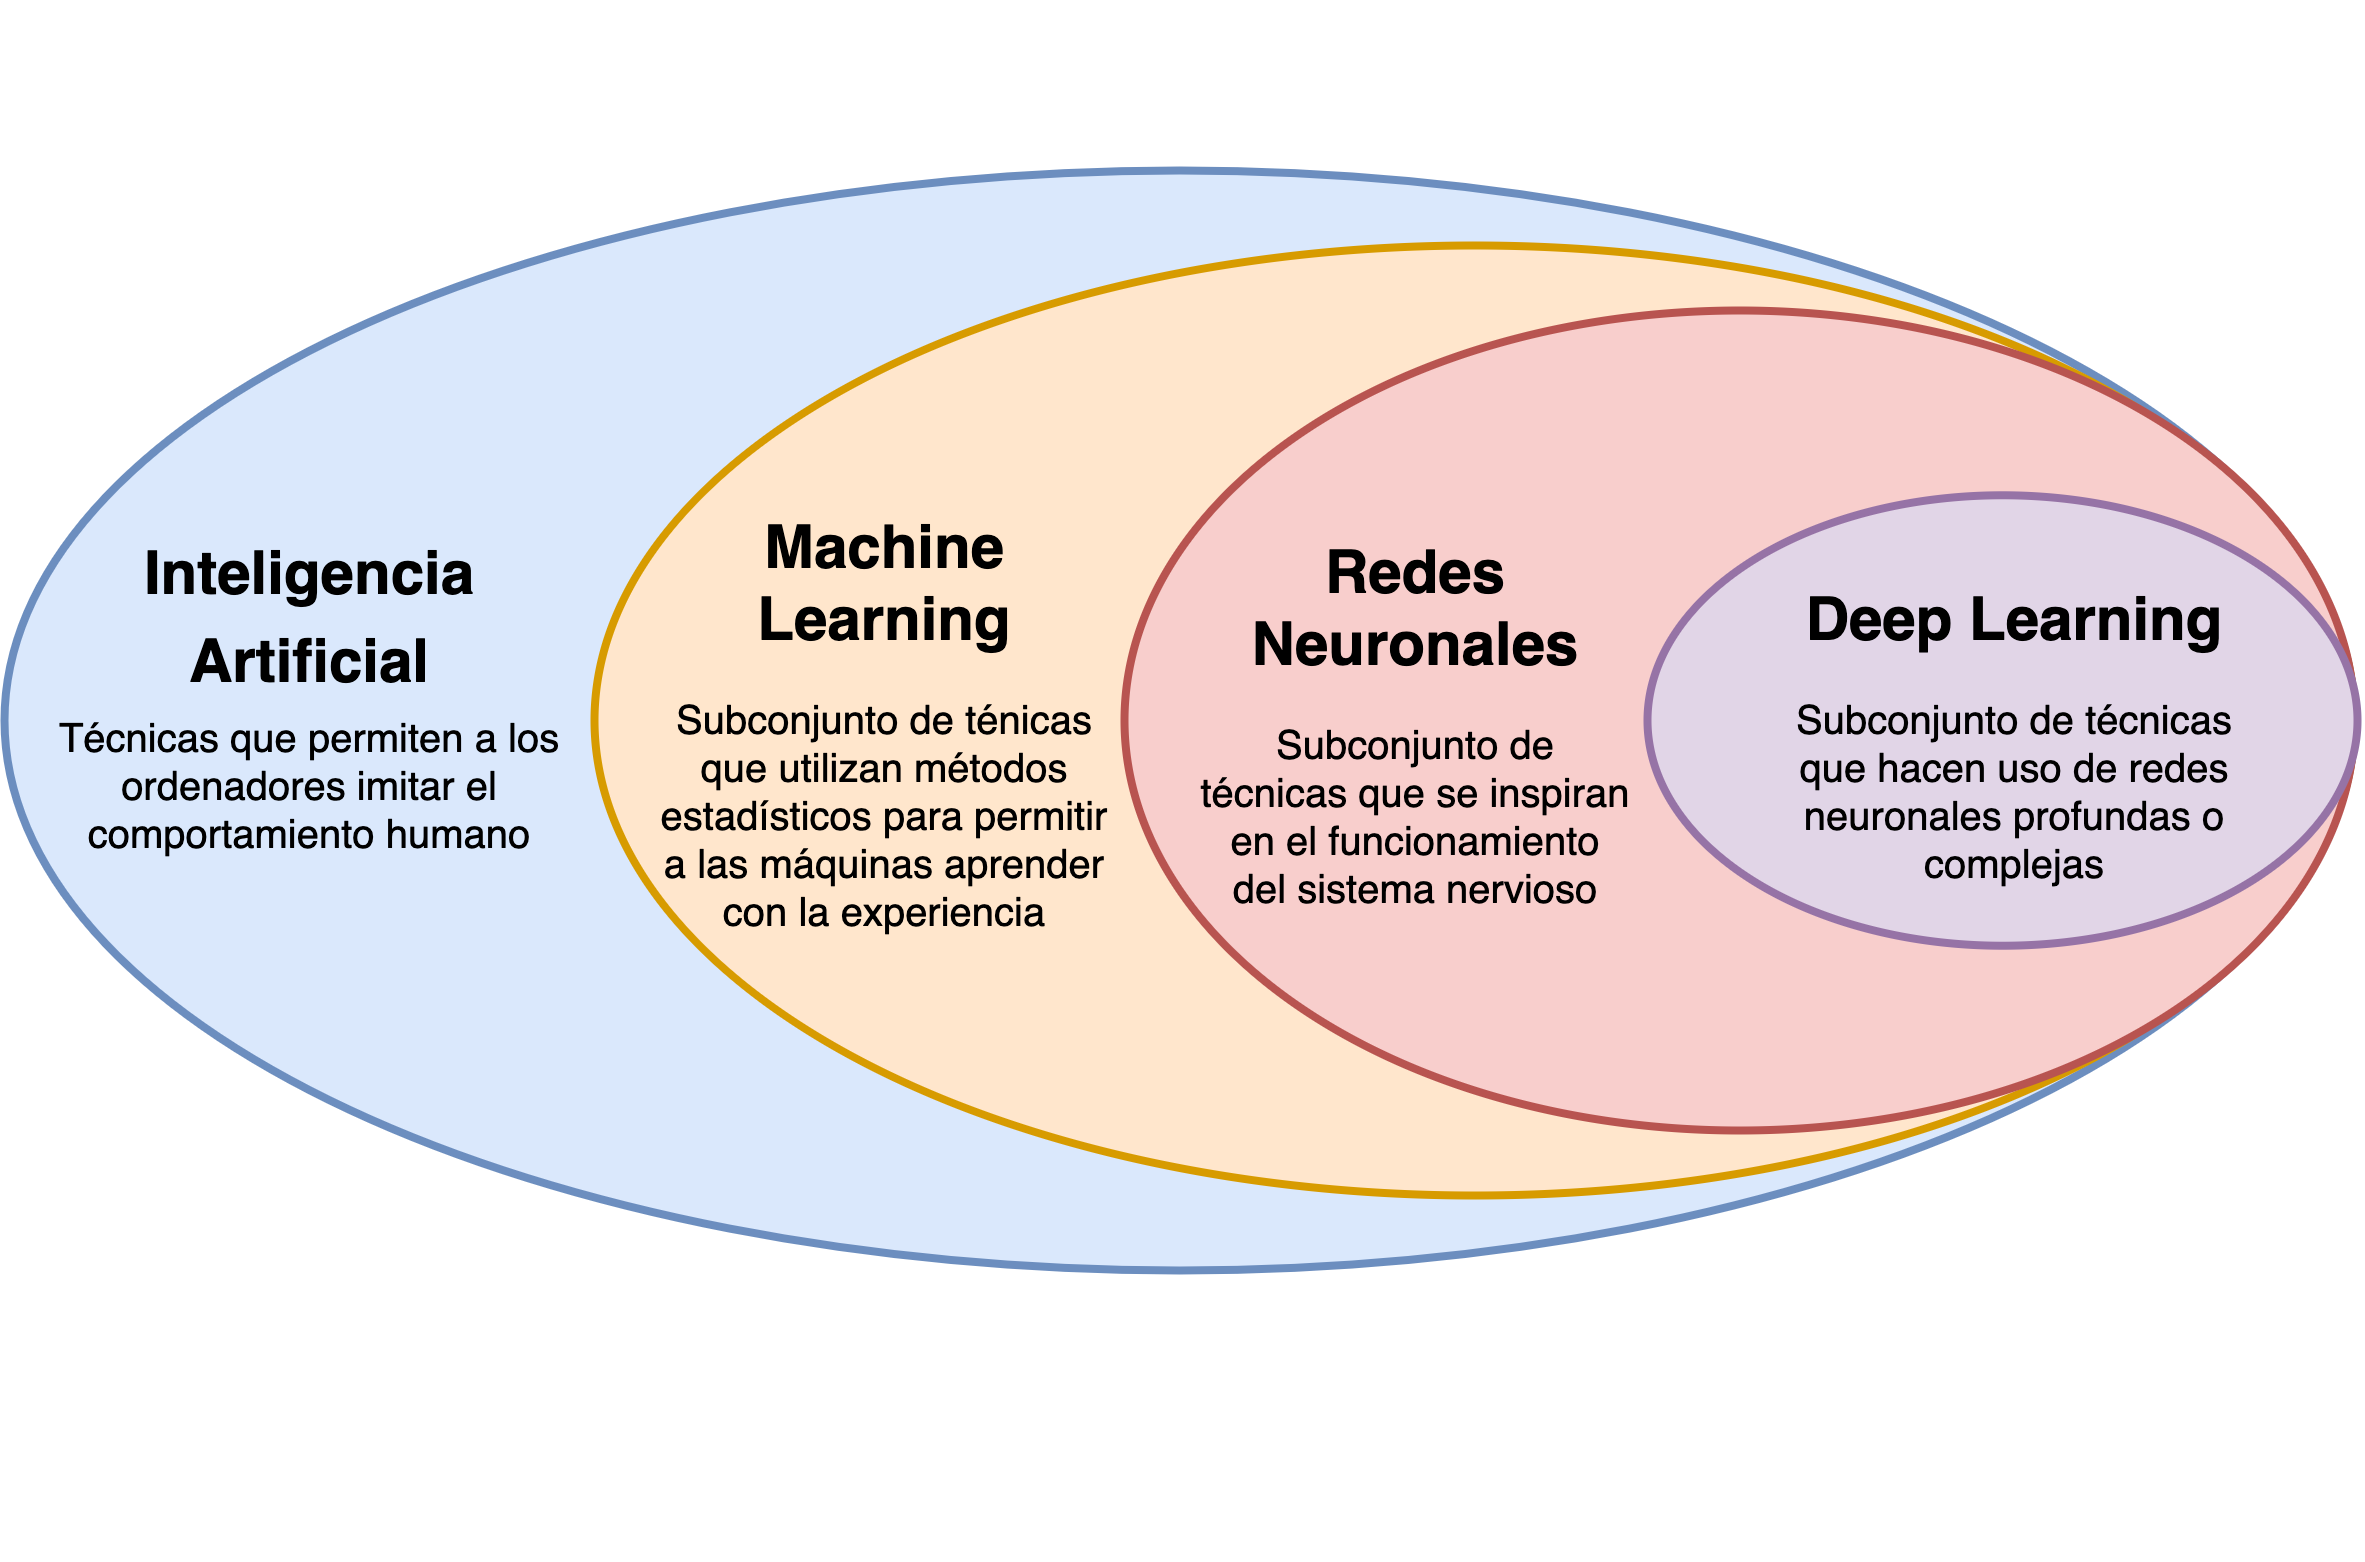
\includegraphics[width=0.5\linewidth,height=\textheight,keepaspectratio]{./imagenes/ia_ml_dl.png}

}

\caption{\label{fig-dl-ml-ai}La inteligencia artificial, el aprendizaje
automático y el deep learning}

\end{figure}%

Matemáticamente, un modelo profundo se puede expresar como una
composición de funciones paramétricas:

\[
f_\theta(\mathbf{x}) = f^{(L)} \circ f^{(L-1)} \circ \cdots \circ f^{(1)}(\mathbf{x})
\]

donde cada \(f^{(l)}\) es una transformación (capa) con parámetros
propios \(\theta^{(l)}\).

La diferencia central respecto de los modelos clásicos es que
\textbf{las representaciones intermedias se aprenden automáticamente} a
partir de los datos, en lugar de ser diseñadas a mano por un experto (lo
que en machine learning clásico se llama \emph{feature engineering}).

\begin{figure}

\centering{

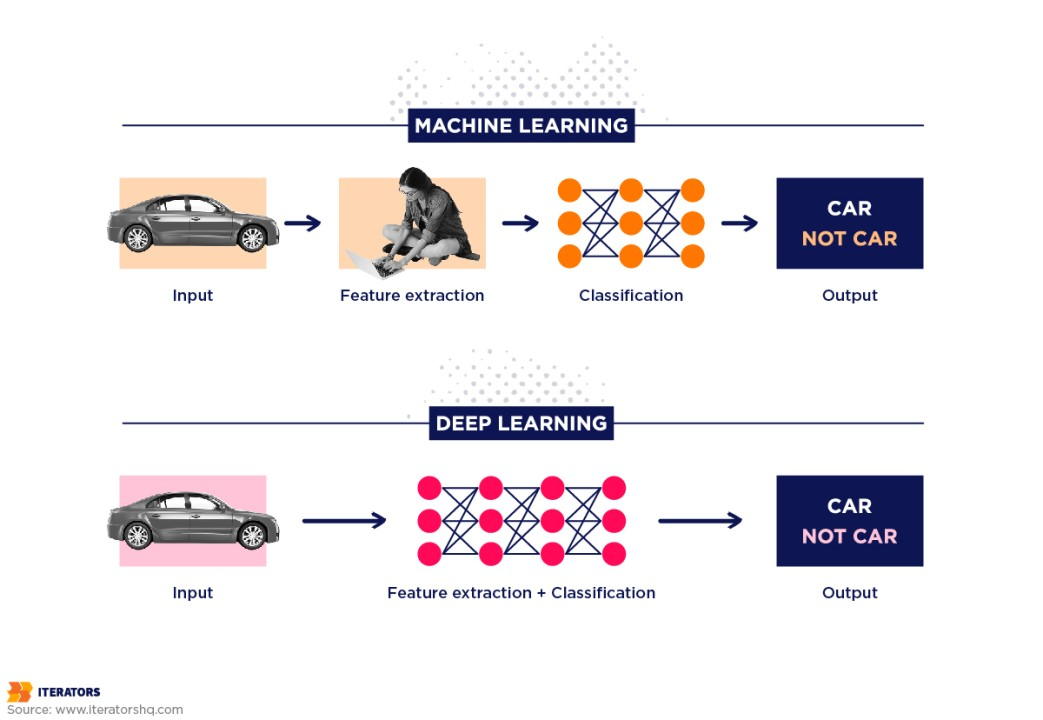
\includegraphics[width=0.5\linewidth,height=\textheight,keepaspectratio]{./imagenes/ml_vs_dl.jpeg}

}

\caption{\label{fig-ml-vs-dl}Machine Learning vs.~Deep Learning}

\end{figure}%

\subsection{Línea de tiempo
histórica}\label{luxednea-de-tiempo-histuxf3rica}

\begin{figure}

\centering{

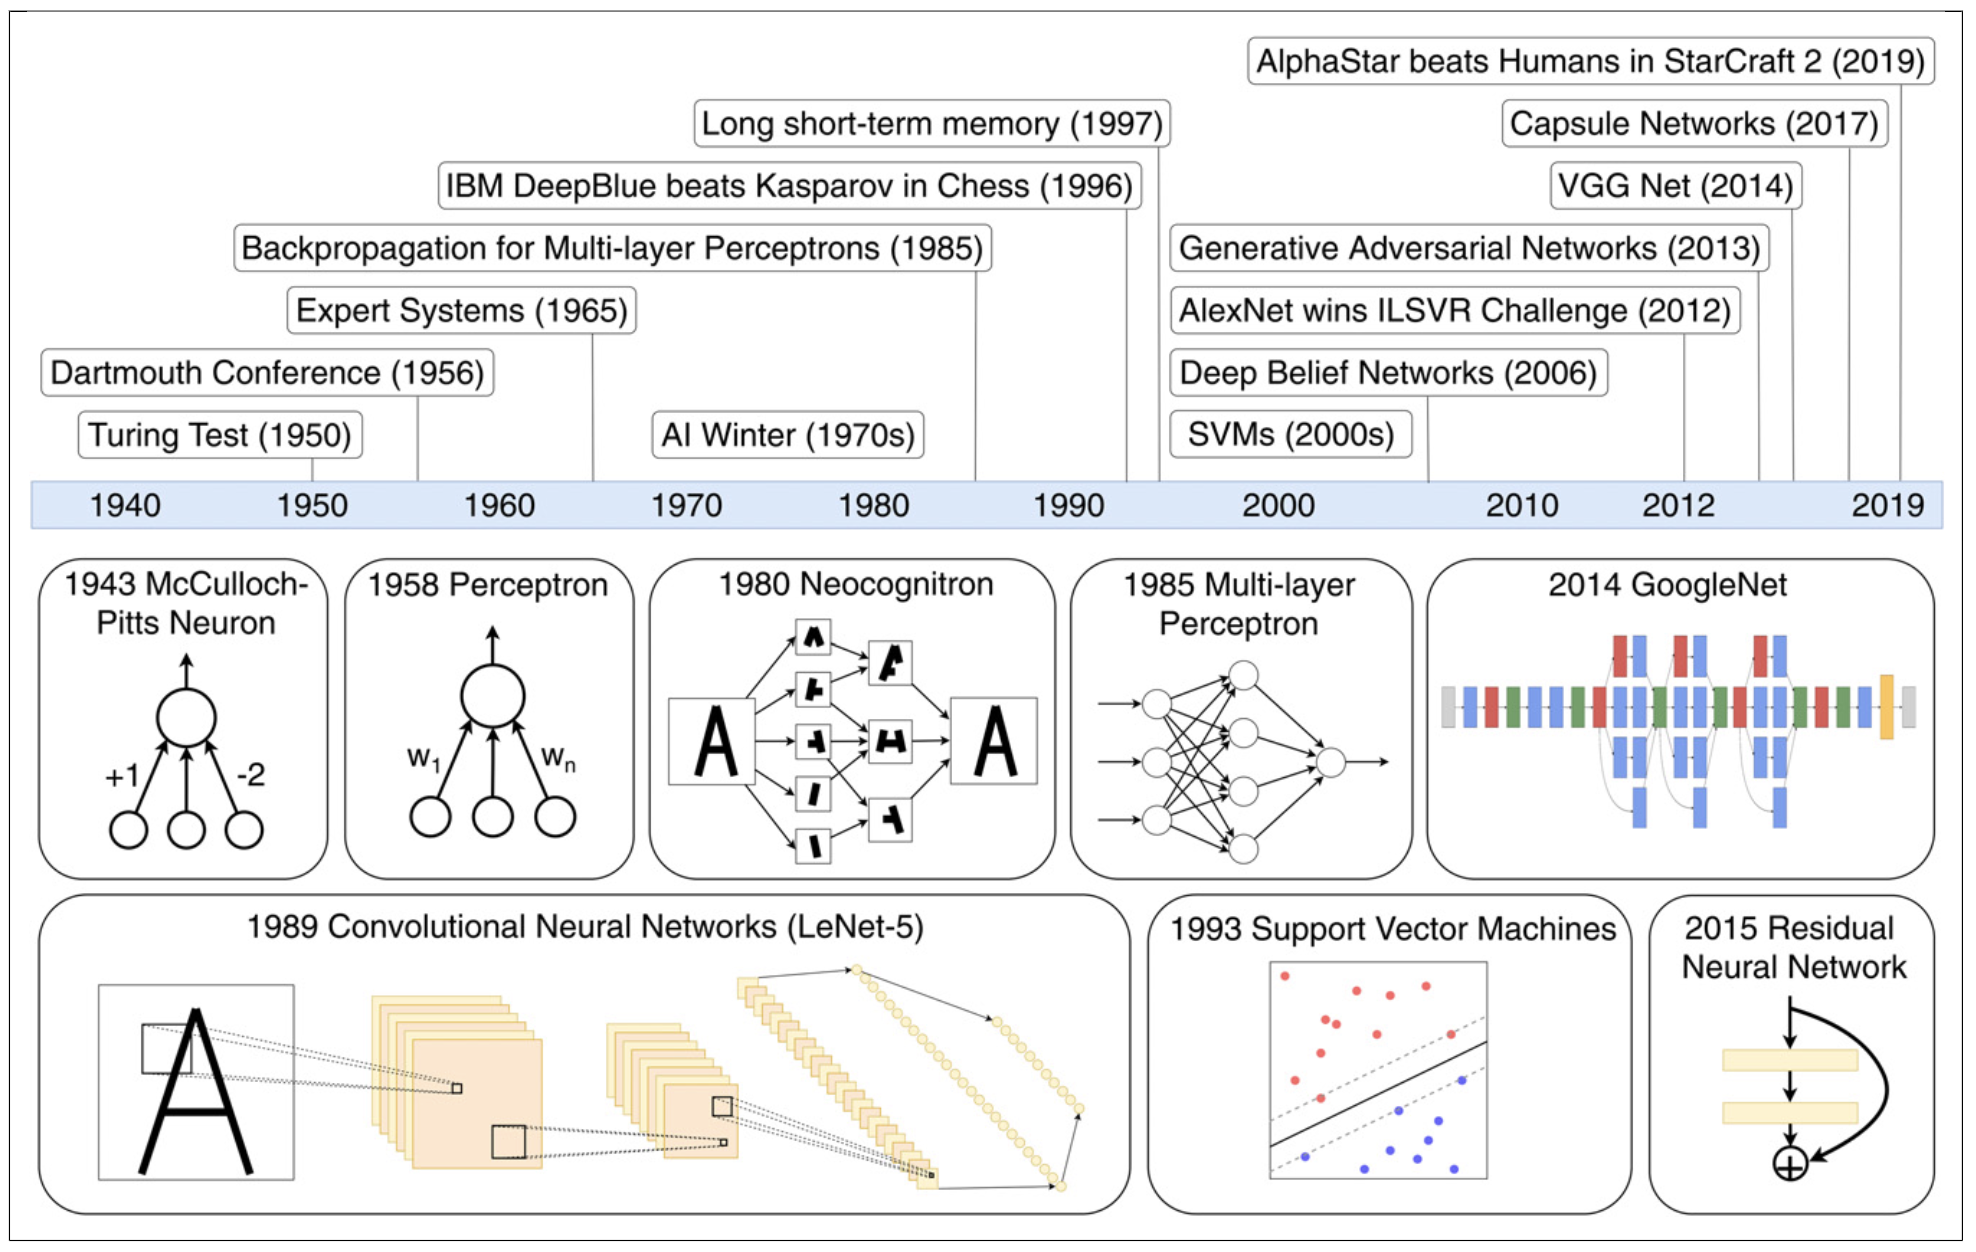
\includegraphics[width=0.8\linewidth,height=\textheight,keepaspectratio]{./imagenes/AI_historia.png}

}

\caption{\label{fig-timeline}Hitos históricos de la IA}

\end{figure}%

La historia del Deep Learning no fue una línea recta: tuvo dos períodos
de estancamiento ---los llamados ``inviernos de la IA''--- separados por
avances puntuales, y un resurgimiento sostenido a partir de 2012 que se
extiende hasta hoy. Repasamos primero esos inviernos y luego, con más
detalle, la década que va de AlexNet (2012) a la actualidad.

\subsection{Los ``dos inviernos'' de la IA
neuronal}\label{los-dos-inviernos-de-la-ia-neuronal}

\begin{enumerate}
\def\labelenumi{\arabic{enumi}.}
\tightlist
\item
  \textbf{Primer invierno (post-1969):} Minsky y Papert demuestran que
  el perceptrón simple no puede resolver problemas no linealmente
  separables (el caso paradigmático: la función XOR, que analizaremos en
  detalle más adelante). Esto reduce drásticamente el financiamiento a
  la investigación en redes neuronales durante casi dos décadas.
\item
  \textbf{Segundo invierno (fines de los 90s-2000s):} a pesar del
  backpropagation (1986), la falta de datos masivos y de poder de
  cómputo, sumada al auge de las SVMs y los métodos de \emph{ensemble},
  relega nuevamente a las redes neuronales.
\item
  \textbf{El resurgimiento (2006-2012):} la disponibilidad de GPUs, de
  grandes bases de datos etiquetadas (ImageNet) y de mejoras
  algorítmicas (ReLU, dropout, mejor inicialización) permite entrenar
  redes verdaderamente profundas. \textbf{AlexNet (2012)} es el punto de
  inflexión que marca el inicio de la era moderna del Deep Learning.
\end{enumerate}

\subsection{ImageNet y el auge de las
CNNs}\label{imagenet-y-el-auge-de-las-cnns}

El \textbf{ImageNet Large Scale Visual Recognition Challenge (ILSVRC)}
fue una competencia anual iniciada en 2010 para evaluar y comparar
algoritmos de reconocimiento visual a gran escala, sobre un subconjunto
de ImageNet de aproximadamente 1.000 clases. Se convirtió en el
benchmark de referencia para medir el progreso en clasificación de
imágenes, y su evolución durante la década de 2010 resume, en una sola
tabla, la revolución de las CNNs:

\begin{itemize}
\tightlist
\item
  \textbf{2010:} el modelo ganador, basado en SVM y características
  tradicionales (HoG, LBP), obtuvo 71,8\% de top-5 accuracy (28,2\% de
  error).
\item
  \textbf{2011:} otro modelo basado en SVM con Fisher Vectors alcanzó
  74,2\% de accuracy (25,0\% de error).
\item
  \textbf{2012:} \textbf{AlexNet}, una CNN profunda, produjo un salto
  abrupto: 84,7\% de accuracy (≈15,3\% de error) --- casi 10 puntos de
  mejora respecto del año anterior.
\item
  \textbf{2013:} las CNNs se consolidan como la estrategia dominante;
  los modelos siguientes superan el 90\% de accuracy.
\item
  \textbf{2014:} arquitecturas como GoogLeNet y VGGNet llevan el
  desempeño a 93-94\% de accuracy.
\item
  \textbf{2015:} \textbf{ResNet} alcanza 96,4\% de accuracy (≈3,6\% de
  error), superando por primera vez el desempeño humano estimado en esta
  tarea.
\item
  \textbf{2016:} CUImage, un \emph{ensemble} de seis redes, roza el 3\%
  de error.
\item
  \textbf{2017:} \textbf{SENet} alcanza el mejor resultado de la
  competencia: 97,75\% de accuracy (2,25\% de error). Los organizadores
  consideran el benchmark esencialmente resuelto y anuncian el final de
  la competencia.
\end{itemize}

En síntesis: entre 2010 y 2017 el error top-5 cayó de 28,2\% a 2,25\%.
El salto más importante ocurrió en 2012 con AlexNet, y marca el comienzo
de la expansión acelerada del deep learning en visión por computadora
--- el mismo AlexNet que abre la línea de tiempo que sigue a
continuación.

\begin{figure}[H]

{\centering \pandocbounded{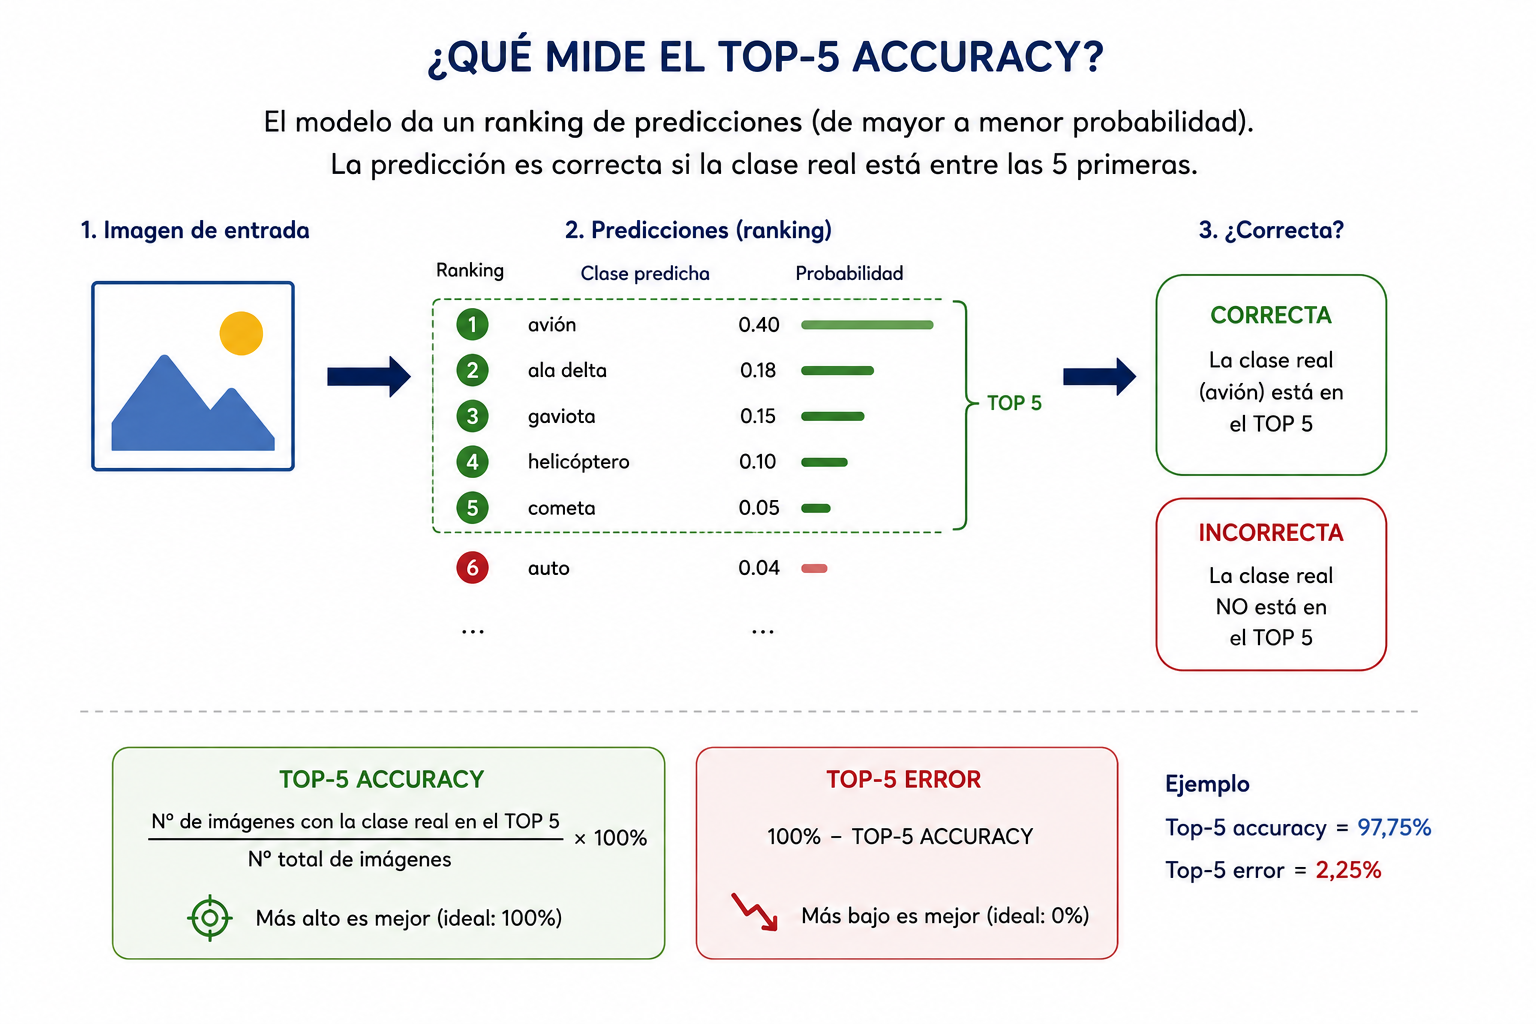
\includegraphics[keepaspectratio]{./imagenes/top5.png}}

}

\caption{Metrica top-5 accuracy}

\end{figure}%

\subsection{Los últimos años: modelos fundacionales y la IA
generativa}\label{los-uxfaltimos-auxf1os-modelos-fundacionales-y-la-ia-generativa}

Desde AlexNet en 2012, el ritmo de avances no hizo más que acelerarse. A
continuación repasamos, año a año, los hitos que llevaron del
``renacimiento'' del deep learning en visión por computadora a los
modelos fundacionales y agénticos actuales, con aplicaciones clínicas
cada vez más concretas en diagnóstico asistido, segmentación automática
y predicción de resultados.

\begin{figure}

\centering{

\includegraphics[width=0.8\linewidth,height=\textheight,keepaspectratio]{./imagenes/10_anos.webp}

}

\caption{\label{fig-recent}Hitos recientes de la IA}

\end{figure}%

\subsubsection{2013 --- AlexNet y los Autoencoders
Variacionales}\label{alexnet-y-los-autoencoders-variacionales}

2013 es considerado el año de ``mayoría de edad'' del deep learning,
consolidando el impacto de AlexNet un año antes. En paralelo surgen los
\textbf{VAEs (Autoencoders Variacionales)}, modelos generativos que
aprenden una representación comprimida (espacio latente) de los datos
para luego generar nuevas muestras, abriendo camino a aplicaciones en
arte, diseño y videojuegos.

\subsubsection{2014 --- Redes Generativas Adversarias
(GANs)}\label{redes-generativas-adversarias-gans}

Ian Goodfellow presenta las \textbf{GANs}: dos redes ---generadora y
discriminadora--- entrenadas en un esquema competitivo, donde una
intenta crear datos sintéticos convincentes y la otra intenta
detectarlos. Se convirtieron rápidamente en una herramienta central para
generar imágenes, video, música y arte, e impulsaron el aprendizaje no
supervisado ---hasta entonces un área poco desarrollada--- al demostrar
que era posible producir datos de alta calidad sin depender de
etiquetas.

\subsubsection{2015 --- ResNets y avances en
NLP}\label{resnets-y-avances-en-nlp}

Kaiming He introduce las \textbf{ResNets}, redes con conexiones
residuales que ``saltean'' capas para resolver el desvanecimiento del
gradiente, permitiendo entrenar redes mucho más profundas de lo que se
creía posible (visto en la tabla de ImageNet más arriba). En paralelo,
las \textbf{RNNs y LSTMs} ---existentes desde los años 90--- empiezan a
rendir gracias a más datos, más cómputo y mejores mecanismos de
\emph{gating}, mejorando traducción automática, generación de texto y
análisis de sentimiento: las bases de los LLMs actuales.

\subsubsection{2016 --- AlphaGo}\label{alphago}

\textbf{AlphaGo}, de DeepMind, derrota al campeón mundial de Go Lee
Sedol, casi dos décadas después de la caída de Kasparov ante Deep Blue
en ajedrez. Combinando aprendizaje por refuerzo profundo con búsqueda
Monte Carlo Tree Search, el sistema evaluó millones de posiciones para
tomar decisiones que superaron la intuición humana en un juego
considerado, hasta entonces, demasiado complejo para las máquinas.

\subsubsection{2017 --- Arquitectura
Transformer}\label{arquitectura-transformer}

El año más determinante de la década. Vaswani y colegas publican
\emph{``Attention Is All You Need''}, introduciendo la
\textbf{arquitectura Transformer}, basada en auto-atención: en vez de
procesar palabras en orden fijo, examina toda la secuencia en
simultáneo, asignando puntajes de relevancia entre palabras. El diseño
encoder-decoder resuelve el problema de las dependencias de largo
alcance que limitaba a las RNNs, y se convierte en el componente base de
todo el desarrollo posterior en NLP y, más adelante, en visión (Unidad
siguiente).

\subsubsection{2018 --- GPT-1, BERT y Graph Neural
Networks}\label{gpt-1-bert-y-graph-neural-networks}

\textbf{OpenAI} lanza \textbf{GPT-1}, demostrando la efectividad de
pre-entrenar de forma no supervisada y luego hacer \emph{fine-tuning} en
tareas específicas. Meses después, \textbf{Google} presenta
\textbf{BERT}, que representa el contexto de cada palabra en ambas
direcciones simultáneamente (no solo hacia adelante, como GPT-1),
superando el estado del arte en múltiples benchmarks de NLP. Ese mismo
año, las \textbf{Graph Neural Networks (GNNs)} ganan tracción aplicando
\emph{message-passing} sobre datos en forma de grafo, con avances en
redes sociales, sistemas de recomendación y descubrimiento de fármacos.

\subsubsection{2019 --- GPT-2 y modelos generativos
mejorados}\label{gpt-2-y-modelos-generativos-mejorados}

\textbf{GPT-2} alcanza desempeño de estado del arte en múltiples tareas
de NLP y genera texto notablemente coherente, anticipando lo que vendría
en los años siguientes. En generación de imágenes, \textbf{BigGAN}
(DeepMind) y \textbf{StyleGAN} (NVIDIA) elevan drásticamente la calidad
y el control sobre las imágenes sintéticas.

\subsubsection{2020 --- GPT-3 y aprendizaje
auto-supervisado}\label{gpt-3-y-aprendizaje-auto-supervisado}

\textbf{GPT-3} representa un salto de escala mayúsculo: de 117 millones
de parámetros (GPT-1) a 1.500 millones (GPT-2) y \textbf{175.000
millones} en GPT-3. Esto le permite generar texto coherente en una
enorme variedad de tareas ---completado, preguntas y respuestas,
escritura creativa--- sin \emph{fine-tuning} específico, poniendo de
relieve el valor del \textbf{aprendizaje auto-supervisado}: entrenar
sobre grandes volúmenes de datos no etiquetados logra una comprensión
amplia del lenguaje de forma mucho más económica que el entrenamiento
supervisado tradicional.

\subsubsection{2021 --- AlphaFold 2, DALL·E y GitHub
Copilot}\label{alphafold-2-dalle-y-github-copilot}

\textbf{AlphaFold 2} (DeepMind) resuelve el problema del plegado de
proteínas extendiendo la arquitectura Transformer, prediciendo la
estructura 3D de una proteína a partir de su secuencia de aminoácidos
--- con enorme potencial para el descubrimiento de fármacos y la
biología estructural. \textbf{DALL·E} (OpenAI) combina modelos de
lenguaje estilo GPT con generación de imágenes a partir de texto,
mientras que \textbf{GitHub Copilot} (con el modelo Codex) lleva la
asistencia de IA a la programación cotidiana.

\subsubsection{2022 --- ChatGPT y Stable
Diffusion}\label{chatgpt-y-stable-diffusion}

\textbf{ChatGPT} (OpenAI, noviembre) lleva los LLMs al público masivo:
conversación fluida, explicaciones, código, distintos estilos de
escritura, todo desde una interfaz simple. Su adopción cruza rápidamente
del ámbito técnico a prácticamente todas las profesiones. En paralelo,
\textbf{Stable Diffusion} (Stability AI) genera imágenes fotorrealistas
desde texto operando en un espacio latente de menor dimensión. Juntos,
disparan una ola masiva de inversión en IA generativa multimodal.

\subsubsection{2023 --- LLMs y bots por todas
partes}\label{llms-y-bots-por-todas-partes}

Cadencia vertiginosa de lanzamientos: \textbf{LLaMA} (Meta, febrero)
supera a GPT-3 con muchos menos parámetros; \textbf{GPT-4} (OpenAI,
marzo) llega multimodal y con capacidades muy superiores;
\textbf{Alpaca} (Stanford) y \textbf{Bard}/\textbf{PaLM-2} (Google)
completan un panorama de competencia intensa entre laboratorios,
mientras la adopción empresarial se acelera (Duolingo Max, Slack GPT,
Shopify, Bing con GPT-4).

\subsubsection{2024 --- La era del razonamiento y la multimodalidad
nativa}\label{la-era-del-razonamiento-y-la-multimodalidad-nativa}

\textbf{OpenAI lanza o1} (septiembre), el primer modelo de
``razonamiento'': entrenado con RL a gran escala para pensar paso a paso
antes de responder, con saltos notables en matemática y programación.
\textbf{GPT-4o} aporta multimodalidad nativa (texto, imagen y audio en
un solo modelo), y OpenAI muestra \textbf{Sora}, capaz de generar video
fotorrealista desde texto. Google presenta \textbf{Gemini} y Meta libera
\textbf{Llama 3}. En el plano regulatorio, la Unión Europea promulga la
\textbf{AI Act}, primer marco normativo integral del mundo para IA.

\subsubsection{2025 --- Razonamiento abierto y el ascenso de los
agentes}\label{razonamiento-abierto-y-el-ascenso-de-los-agentes}

\textbf{DeepSeek-R1} (enero) iguala el desempeño de o1 con una fracción
del costo de entrenamiento, consolidando a China como competidor de
primer nivel en modelos abiertos. OpenAI responde con \textbf{o3}, y los
laboratorios grandes (Google, Anthropic, Meta, Alibaba) lanzan sus
propias familias de modelos de razonamiento. El foco se desplaza de
``modelos que responden'' a \textbf{agentes que actúan}: Claude 4/4.5 y
herramientas como Claude Code o Cursor permiten delegar tareas de
programación completas. Google presenta \textbf{Gemini 3}, primer modelo
en superar 1500 Elo en LMArena.

\subsubsection{2026 --- El ascenso de China}\label{el-ascenso-de-china}

China se posiciona como líder global en investigación y desarrollo de
IA, con avances importantes en modelos de lenguaje, visión por
computadora y sistemas de razonamiento. La inversión estatal y el
ecosistema empresarial local aceleran la innovación, consolidando al
país como un actor central en la evolución de la inteligencia
artificial. \textbf{Kimi K3}, un modelo de pesos abiertos desarrollado
por \textbf{Moonshot AI} con cerca de 3 billones de parámetros
(arquitectura \emph{mixture-of-experts}), se posiciona al mismo nivel
que GPT-5 o Gemini 3 en varios benchmarks --- un nuevo capítulo en la
democratización de la inteligencia artificial.

\subsection{¿Por qué ``profundo'' y por qué ahora es relevante en Física
Médica?}\label{por-quuxe9-profundo-y-por-quuxe9-ahora-es-relevante-en-fuxedsica-muxe9dica}

\begin{itemize}
\tightlist
\item
  \textbf{Datos:} las imágenes médicas (CT, RM, PET, mamografía) son
  datos de alta dimensionalidad donde el Deep Learning ---en particular
  las CNNs--- sobresale.
\item
  \textbf{Cómputo:} las GPUs/TPUs permiten entrenar modelos con millones
  de parámetros en tiempos razonables.
\item
  \textbf{Representaciones jerárquicas:} en imágenes médicas, las capas
  iniciales aprenden bordes y texturas; las capas intermedias,
  estructuras anatómicas; las capas profundas, patrones patológicos
  complejos (una analogía directa con la vía visual biológica).
\end{itemize}

\begin{tcolorbox}[enhanced jigsaw, arc=.35mm, bottomrule=.15mm, bottomtitle=1mm, breakable, colback=white, colbacktitle=quarto-callout-tip-color!10!white, colframe=quarto-callout-tip-color-frame, coltitle=black, left=2mm, leftrule=.75mm, opacityback=0, opacitybacktitle=0.6, rightrule=.15mm, title=\textcolor{quarto-callout-tip-color}{\faLightbulb}\hspace{0.5em}{Aplicaciones actuales en Física Médica}, titlerule=0mm, toprule=.15mm, toptitle=1mm]

\begin{itemize}
\tightlist
\item
  Segmentación automática de órganos en riesgo (OARs) y tumores
\item
  Reducción de dosis en CT mediante \emph{denoising} con redes profundas
\item
  Reconstrucción de imágenes PET/RM aceleradas
\item
  Detección asistida de nódulos, lesiones y contornos tumorales
\item
  Control de calidad automatizado y predicción de \emph{outcomes}
  clínicos
\end{itemize}

\end{tcolorbox}

\begin{center}\rule{0.5\linewidth}{0.5pt}\end{center}

\section{Redes neuronales simples: el algoritmo del
Perceptrón}\label{redes-neuronales-simples-el-algoritmo-del-perceptruxf3n}

\subsection{La neurona biológica como
inspiración}\label{la-neurona-bioluxf3gica-como-inspiraciuxf3n}

McCulloch y Pitts (1943) propusieron un modelo matemático simplificado
de la neurona: recibe señales de entrada, las pondera y produce una
salida binaria si supera un umbral. Con ese modelo mostraron que una red
de neuronas simples podía implementar cualquier función lógica booleana.
Rosenblatt (1958) retomó esa idea y la convirtió en un \textbf{algoritmo
de aprendizaje} capaz de ajustar los pesos automáticamente a partir de
ejemplos: el Perceptrón.

\subsection{Definición formal}\label{definiciuxf3n-formal}

Dado un vector de entrada
\(\mathbf{x} = (x_1, x_2, \dots, x_d) \in \mathbb{R}^d\), el perceptrón
calcula:

\[
z = \sum_{j=1}^{d} w_j x_j + b = \mathbf{w}^\top \mathbf{x} + b
\]

\[
\hat{y} = \phi(z) = 
\begin{cases}
1 & \text{si } z \geq 0 \\
0 \text{ (ó } -1) & \text{si } z < 0
\end{cases}
\]

donde \(\phi\) es la \textbf{función de activación escalón (Heaviside)},
\(\mathbf{w}\) es el vector de pesos sinápticos y \(b\) el sesgo
(\emph{bias}).

Geométricamente, el perceptrón define un \textbf{hiperplano separador}
en \(\mathbb{R}^d\): \(\mathbf{w}^\top \mathbf{x} + b = 0\). Todo lo que
quede de un lado del hiperplano se clasifica como \(+1\); todo lo que
quede del otro lado, como \(-1\) (o \(0\)). Esta lectura geométrica es
la clave para entender, en la próxima sección, qué puede y qué no puede
aprender un único perceptrón.

\subsection{El algoritmo de aprendizaje del
Perceptrón}\label{el-algoritmo-de-aprendizaje-del-perceptruxf3n}

Dado un conjunto de entrenamiento \(\{(\mathbf{x}_i, y_i)\}_{i=1}^N\)
con \(y_i \in \{-1, +1\}\), el algoritmo actualiza los pesos
\textbf{solo cuando comete un error}:

\textbf{Algoritmo (Rosenblatt, 1958):}

\begin{enumerate}
\def\labelenumi{\arabic{enumi}.}
\tightlist
\item
  Inicializar \(\mathbf{w} \leftarrow \mathbf{0}\), \(b \leftarrow 0\)
\item
  Repetir hasta convergencia (o número máximo de épocas): Para cada
  \((\mathbf{x}_i, y_i)\):

  \begin{itemize}
  \tightlist
  \item
    Calcular
    \(\hat{y}_i = \text{sign}(\mathbf{w}^\top \mathbf{x}_i + b)\)
  \item
    Si \(\hat{y}_i \neq y_i\): \[
    \mathbf{w} \leftarrow \mathbf{w} + \eta \, y_i \, \mathbf{x}_i, \qquad b \leftarrow b + \eta \, y_i
    \]
  \end{itemize}
\end{enumerate}

donde \(\eta > 0\) es la tasa de aprendizaje (\emph{learning rate}).

\begin{tcolorbox}[enhanced jigsaw, arc=.35mm, bottomrule=.15mm, bottomtitle=1mm, breakable, colback=white, colbacktitle=quarto-callout-important-color!10!white, colframe=quarto-callout-important-color-frame, coltitle=black, left=2mm, leftrule=.75mm, opacityback=0, opacitybacktitle=0.6, rightrule=.15mm, title=\textcolor{quarto-callout-important-color}{\faExclamation}\hspace{0.5em}{Teorema de convergencia del Perceptrón}, titlerule=0mm, toprule=.15mm, toptitle=1mm]

Si los datos son \textbf{linealmente separables}, el algoritmo del
perceptrón converge en un número finito de pasos a una solución que
clasifica correctamente todo el conjunto de entrenamiento (Novikoff,
1962). Si los datos \textbf{no} son linealmente separables, el algoritmo
\textbf{nunca converge} y oscila indefinidamente. La siguiente sección
muestra ambos casos en la práctica.

\end{tcolorbox}

\subsection{Implementación desde
cero}\label{implementaciuxf3n-desde-cero}

\protect\phantomsection\label{perceptron-impl}
\begin{Shaded}
\begin{Highlighting}[]
\ImportTok{import}\NormalTok{ numpy }\ImportTok{as}\NormalTok{ np}

\KeywordTok{class}\NormalTok{ Perceptron:}
    \KeywordTok{def} \FunctionTok{\_\_init\_\_}\NormalTok{(}\VariableTok{self}\NormalTok{, lr}\OperatorTok{=}\FloatTok{0.1}\NormalTok{, n\_epochs}\OperatorTok{=}\DecValTok{50}\NormalTok{):}
        \VariableTok{self}\NormalTok{.lr }\OperatorTok{=}\NormalTok{ lr}
        \VariableTok{self}\NormalTok{.n\_epochs }\OperatorTok{=}\NormalTok{ n\_epochs}

    \KeywordTok{def}\NormalTok{ fit(}\VariableTok{self}\NormalTok{, X, y):}
\NormalTok{        n\_samples, n\_features }\OperatorTok{=}\NormalTok{ X.shape}
        \VariableTok{self}\NormalTok{.w }\OperatorTok{=}\NormalTok{ np.zeros(n\_features)}
        \VariableTok{self}\NormalTok{.b }\OperatorTok{=} \FloatTok{0.0}
        \VariableTok{self}\NormalTok{.errores\_por\_epoca }\OperatorTok{=}\NormalTok{ []}

        \ControlFlowTok{for}\NormalTok{ epoca }\KeywordTok{in} \BuiltInTok{range}\NormalTok{(}\VariableTok{self}\NormalTok{.n\_epochs):}
\NormalTok{            errores }\OperatorTok{=} \DecValTok{0}
            \ControlFlowTok{for}\NormalTok{ xi, yi }\KeywordTok{in} \BuiltInTok{zip}\NormalTok{(X, y):}
\NormalTok{                y\_pred }\OperatorTok{=}\NormalTok{ np.sign(np.dot(}\VariableTok{self}\NormalTok{.w, xi) }\OperatorTok{+} \VariableTok{self}\NormalTok{.b)}
\NormalTok{                y\_pred }\OperatorTok{=} \DecValTok{1} \ControlFlowTok{if}\NormalTok{ y\_pred }\OperatorTok{\textgreater{}=} \DecValTok{0} \ControlFlowTok{else} \OperatorTok{{-}}\DecValTok{1}
                \ControlFlowTok{if}\NormalTok{ y\_pred }\OperatorTok{!=}\NormalTok{ yi:}
                    \VariableTok{self}\NormalTok{.w }\OperatorTok{+=} \VariableTok{self}\NormalTok{.lr }\OperatorTok{*}\NormalTok{ yi }\OperatorTok{*}\NormalTok{ xi}
                    \VariableTok{self}\NormalTok{.b }\OperatorTok{+=} \VariableTok{self}\NormalTok{.lr }\OperatorTok{*}\NormalTok{ yi}
\NormalTok{                    errores }\OperatorTok{+=} \DecValTok{1}
            \VariableTok{self}\NormalTok{.errores\_por\_epoca.append(errores)}
            \ControlFlowTok{if}\NormalTok{ errores }\OperatorTok{==} \DecValTok{0}\NormalTok{:}
                \ControlFlowTok{break}
        \ControlFlowTok{return} \VariableTok{self}

    \KeywordTok{def}\NormalTok{ predict(}\VariableTok{self}\NormalTok{, X):}
\NormalTok{        z }\OperatorTok{=}\NormalTok{ X }\OperatorTok{@} \VariableTok{self}\NormalTok{.w }\OperatorTok{+} \VariableTok{self}\NormalTok{.b}
        \ControlFlowTok{return}\NormalTok{ np.where(z }\OperatorTok{\textgreater{}=} \DecValTok{0}\NormalTok{, }\DecValTok{1}\NormalTok{, }\OperatorTok{{-}}\DecValTok{1}\NormalTok{)}
\end{Highlighting}
\end{Shaded}

\subsection{Ejemplo: separación de dos clases sintéticas (linealmente
separables)}\label{ejemplo-separaciuxf3n-de-dos-clases-sintuxe9ticas-linealmente-separables}

\begin{figure}

\centering{

\begin{Shaded}
\begin{Highlighting}[]
\ImportTok{import}\NormalTok{ matplotlib.pyplot }\ImportTok{as}\NormalTok{ plt}
\ImportTok{from}\NormalTok{ sklearn.datasets }\ImportTok{import}\NormalTok{ make\_blobs}

\NormalTok{X, y }\OperatorTok{=}\NormalTok{ make\_blobs(n\_samples}\OperatorTok{=}\DecValTok{100}\NormalTok{, centers}\OperatorTok{=}\DecValTok{2}\NormalTok{, cluster\_std}\OperatorTok{=}\FloatTok{1.0}\NormalTok{, random\_state}\OperatorTok{=}\DecValTok{7}\NormalTok{)}
\NormalTok{y }\OperatorTok{=}\NormalTok{ np.where(y }\OperatorTok{==} \DecValTok{0}\NormalTok{, }\OperatorTok{{-}}\DecValTok{1}\NormalTok{, }\DecValTok{1}\NormalTok{)}

\NormalTok{modelo }\OperatorTok{=}\NormalTok{ Perceptron(lr}\OperatorTok{=}\FloatTok{0.1}\NormalTok{, n\_epochs}\OperatorTok{=}\DecValTok{30}\NormalTok{).fit(X, y)}

\NormalTok{fig, axes }\OperatorTok{=}\NormalTok{ plt.subplots(}\DecValTok{1}\NormalTok{, }\DecValTok{2}\NormalTok{, figsize}\OperatorTok{=}\NormalTok{(}\DecValTok{11}\NormalTok{, }\FloatTok{4.2}\NormalTok{))}

\CommentTok{\# Frontera de decisión}
\NormalTok{xx, yy }\OperatorTok{=}\NormalTok{ np.meshgrid(np.linspace(X[:,}\DecValTok{0}\NormalTok{].}\BuiltInTok{min}\NormalTok{()}\OperatorTok{{-}}\DecValTok{1}\NormalTok{, X[:,}\DecValTok{0}\NormalTok{].}\BuiltInTok{max}\NormalTok{()}\OperatorTok{+}\DecValTok{1}\NormalTok{, }\DecValTok{200}\NormalTok{),}
\NormalTok{                      np.linspace(X[:,}\DecValTok{1}\NormalTok{].}\BuiltInTok{min}\NormalTok{()}\OperatorTok{{-}}\DecValTok{1}\NormalTok{, X[:,}\DecValTok{1}\NormalTok{].}\BuiltInTok{max}\NormalTok{()}\OperatorTok{+}\DecValTok{1}\NormalTok{, }\DecValTok{200}\NormalTok{))}
\NormalTok{Z }\OperatorTok{=}\NormalTok{ modelo.predict(np.c\_[xx.ravel(), yy.ravel()]).reshape(xx.shape)}
\NormalTok{axes[}\DecValTok{0}\NormalTok{].contourf(xx, yy, Z, alpha}\OperatorTok{=}\FloatTok{0.3}\NormalTok{, cmap}\OperatorTok{=}\StringTok{"coolwarm"}\NormalTok{)}
\NormalTok{axes[}\DecValTok{0}\NormalTok{].scatter(X[:,}\DecValTok{0}\NormalTok{], X[:,}\DecValTok{1}\NormalTok{], c}\OperatorTok{=}\NormalTok{y, cmap}\OperatorTok{=}\StringTok{"coolwarm"}\NormalTok{, edgecolor}\OperatorTok{=}\StringTok{"k"}\NormalTok{)}
\NormalTok{axes[}\DecValTok{0}\NormalTok{].set\_title(}\StringTok{"Frontera de decisión aprendida"}\NormalTok{)}

\CommentTok{\# Curva de convergencia}
\NormalTok{axes[}\DecValTok{1}\NormalTok{].plot(modelo.errores\_por\_epoca, marker}\OperatorTok{=}\StringTok{"o"}\NormalTok{, color}\OperatorTok{=}\StringTok{"darkred"}\NormalTok{)}
\NormalTok{axes[}\DecValTok{1}\NormalTok{].set\_xlabel(}\StringTok{"Época"}\NormalTok{)}
\NormalTok{axes[}\DecValTok{1}\NormalTok{].set\_ylabel(}\StringTok{"N° de errores de clasificación"}\NormalTok{)}
\NormalTok{axes[}\DecValTok{1}\NormalTok{].set\_title(}\StringTok{"Convergencia del algoritmo"}\NormalTok{)}
\NormalTok{axes[}\DecValTok{1}\NormalTok{].grid(alpha}\OperatorTok{=}\FloatTok{0.3}\NormalTok{)}

\NormalTok{plt.tight\_layout()}
\NormalTok{plt.show()}
\end{Highlighting}
\end{Shaded}

}

\caption{\label{fig-perceptron-separable}}

\end{figure}%

\subsection{De funciones lógicas simples a XOR: qué separa un perceptrón
y qué
no}\label{de-funciones-luxf3gicas-simples-a-xor-quuxe9-separa-un-perceptruxf3n-y-quuxe9-no}

Antes de llegar al límite del perceptrón conviene ver, en detalle, en
qué tipo de problemas sí funciona --- y por qué. La forma más simple de
probar un clasificador binario con dos entradas es pedirle que aprenda
una \textbf{función lógica booleana}: AND, OR, NAND, NOR y, finalmente,
XOR. Todas ellas toman dos entradas \(x_1, x_2 \in \{0,1\}\) y devuelven
una salida binaria, y todas caben en un plano de dos dimensiones --- lo
que las vuelve ideales para visualizar qué significa ``ser linealmente
separable''.

\subsubsection{AND, OR, NAND, NOR: linealmente
separables}\label{and-or-nand-nor-linealmente-separables}

Las siguientes tablas de verdad definen las funciones AND, OR, NAND y
NOR:

{\def\LTcaptype{none} % do not increment counter
\begin{longtable}[]{@{}llllll@{}}
\toprule\noalign{}
\(x_1\) & \(x_2\) & AND & OR & NAND & NOR \\
\midrule\noalign{}
\endhead
\bottomrule\noalign{}
\endlastfoot
0 & 0 & 0 & 0 & 1 & 1 \\
0 & 1 & 0 & 1 & 1 & 0 \\
1 & 0 & 0 & 1 & 1 & 0 \\
1 & 1 & 1 & 1 & 0 & 0 \\
\end{longtable}
}

Para cada una de estas funciones existe un hiperplano (en este caso, una
recta en \(\mathbb{R}^2\)) que separa perfectamente los puntos de salida
\(1\) de los de salida \(0\). Basta con encontrar \(w_1, w_2, b\)
adecuados. Algunos ejemplos que un perceptrón puede encontrar (no son
los únicos posibles):

\begin{itemize}
\tightlist
\item
  \textbf{AND:} \(w_1 = w_2 = 1\), \(b = -1.5\) → solo \((1,1)\) supera
  el umbral de \(z \geq 0\).
\item
  \textbf{OR:} \(w_1 = w_2 = 1\), \(b = -0.5\) → cualquier entrada con
  al menos un \(1\) supera el umbral.
\item
  \textbf{NAND} (NOT AND): \(w_1 = w_2 = -1\), \(b = 1.5\) → el negado
  exacto de AND.
\item
  \textbf{NOR} (NOT OR): \(w_1 = w_2 = -1\), \(b = 0.5\) → el negado
  exacto de OR.
\end{itemize}

El siguiente código entrena un perceptrón real ---el mismo implementado
más arriba--- sobre cada una de estas funciones, y confirma que converge
sin errores en las cuatro:

\begin{figure}

\centering{

\begin{Shaded}
\begin{Highlighting}[]
\NormalTok{X\_bool }\OperatorTok{=}\NormalTok{ np.array([[}\DecValTok{0}\NormalTok{,}\DecValTok{0}\NormalTok{],[}\DecValTok{0}\NormalTok{,}\DecValTok{1}\NormalTok{],[}\DecValTok{1}\NormalTok{,}\DecValTok{0}\NormalTok{],[}\DecValTok{1}\NormalTok{,}\DecValTok{1}\NormalTok{]])}
\NormalTok{compuertas }\OperatorTok{=}\NormalTok{ \{}
    \StringTok{"AND"}\NormalTok{:  np.array([}\OperatorTok{{-}}\DecValTok{1}\NormalTok{,}\OperatorTok{{-}}\DecValTok{1}\NormalTok{,}\OperatorTok{{-}}\DecValTok{1}\NormalTok{, }\DecValTok{1}\NormalTok{]),}
    \StringTok{"OR"}\NormalTok{:   np.array([}\OperatorTok{{-}}\DecValTok{1}\NormalTok{, }\DecValTok{1}\NormalTok{, }\DecValTok{1}\NormalTok{, }\DecValTok{1}\NormalTok{]),}
    \StringTok{"NAND"}\NormalTok{: np.array([ }\DecValTok{1}\NormalTok{, }\DecValTok{1}\NormalTok{, }\DecValTok{1}\NormalTok{,}\OperatorTok{{-}}\DecValTok{1}\NormalTok{]),}
    \StringTok{"NOR"}\NormalTok{:  np.array([ }\DecValTok{1}\NormalTok{,}\OperatorTok{{-}}\DecValTok{1}\NormalTok{,}\OperatorTok{{-}}\DecValTok{1}\NormalTok{,}\OperatorTok{{-}}\DecValTok{1}\NormalTok{]),}
\NormalTok{\}}

\NormalTok{fig, axes }\OperatorTok{=}\NormalTok{ plt.subplots(}\DecValTok{1}\NormalTok{, }\DecValTok{4}\NormalTok{, figsize}\OperatorTok{=}\NormalTok{(}\DecValTok{16}\NormalTok{, }\DecValTok{4}\NormalTok{))}
\NormalTok{xx\_b, yy\_b }\OperatorTok{=}\NormalTok{ np.meshgrid(np.linspace(}\OperatorTok{{-}}\FloatTok{0.5}\NormalTok{, }\FloatTok{1.5}\NormalTok{, }\DecValTok{200}\NormalTok{), np.linspace(}\OperatorTok{{-}}\FloatTok{0.5}\NormalTok{, }\FloatTok{1.5}\NormalTok{, }\DecValTok{200}\NormalTok{))}

\ControlFlowTok{for}\NormalTok{ ax, (nombre, y\_gate) }\KeywordTok{in} \BuiltInTok{zip}\NormalTok{(axes, compuertas.items()):}
\NormalTok{    modelo\_gate }\OperatorTok{=}\NormalTok{ Perceptron(lr}\OperatorTok{=}\FloatTok{0.5}\NormalTok{, n\_epochs}\OperatorTok{=}\DecValTok{50}\NormalTok{).fit(X\_bool, y\_gate)}
\NormalTok{    Z }\OperatorTok{=}\NormalTok{ modelo\_gate.predict(np.c\_[xx\_b.ravel(), yy\_b.ravel()]).reshape(xx\_b.shape)}
\NormalTok{    ax.contourf(xx\_b, yy\_b, Z, alpha}\OperatorTok{=}\FloatTok{0.3}\NormalTok{, cmap}\OperatorTok{=}\StringTok{"coolwarm"}\NormalTok{)}
\NormalTok{    ax.scatter(X\_bool[:,}\DecValTok{0}\NormalTok{], X\_bool[:,}\DecValTok{1}\NormalTok{], c}\OperatorTok{=}\NormalTok{y\_gate, cmap}\OperatorTok{=}\StringTok{"coolwarm"}\NormalTok{, s}\OperatorTok{=}\DecValTok{150}\NormalTok{, edgecolor}\OperatorTok{=}\StringTok{"k"}\NormalTok{)}
\NormalTok{    convergio }\OperatorTok{=} \StringTok{"sí"} \ControlFlowTok{if}\NormalTok{ modelo\_gate.errores\_por\_epoca[}\OperatorTok{{-}}\DecValTok{1}\NormalTok{] }\OperatorTok{==} \DecValTok{0} \ControlFlowTok{else} \StringTok{"no"}
\NormalTok{    ax.set\_title(}\SpecialStringTok{f"}\SpecialCharTok{\{}\NormalTok{nombre}\SpecialCharTok{\}}\SpecialStringTok{ (converge: }\SpecialCharTok{\{}\NormalTok{convergio}\SpecialCharTok{\}}\SpecialStringTok{)"}\NormalTok{, fontsize}\OperatorTok{=}\DecValTok{11}\NormalTok{)}
\NormalTok{    ax.set\_xticks([}\DecValTok{0}\NormalTok{,}\DecValTok{1}\NormalTok{])}\OperatorTok{;}\NormalTok{ ax.set\_yticks([}\DecValTok{0}\NormalTok{,}\DecValTok{1}\NormalTok{])}

\NormalTok{plt.tight\_layout()}
\NormalTok{plt.show()}
\end{Highlighting}
\end{Shaded}

}

\caption{\label{fig-compuertas-logicas}}

\end{figure}%

En los cuatro casos aparece una recta que separa limpiamente ambas
clases, y el algoritmo converge en pocas épocas --- tal como predice el
teorema de Novikoff.

\subsubsection{El límite fundamental: el problema
XOR}\label{el-luxedmite-fundamental-el-problema-xor}

La función \textbf{XOR} (OR exclusivo) es la excepción:

{\def\LTcaptype{none} % do not increment counter
\begin{longtable}[]{@{}lll@{}}
\toprule\noalign{}
\(x_1\) & \(x_2\) & XOR \\
\midrule\noalign{}
\endhead
\bottomrule\noalign{}
\endlastfoot
0 & 0 & 0 \\
0 & 1 & 1 \\
1 & 0 & 1 \\
1 & 1 & 0 \\
\end{longtable}
}

A diferencia de AND/OR/NAND/NOR, aquí las dos clases están
\textbf{entrelazadas geométricamente}: los puntos \((0,0)\) y \((1,1)\)
pertenecen a una clase, mientras que \((0,1)\) y \((1,0)\) ---sus
``vecinos'' más cercanos en el plano--- pertenecen a la otra. No existe
ninguna recta capaz de dejar a \((0,0)\) y \((1,1)\) de un lado y a
\((0,1)\) y \((1,0)\) del otro: cualquier línea que separe correctamente
dos de los cuatro puntos, deja mal clasificado a algún tercero.

\begin{figure}

\centering{

\begin{Shaded}
\begin{Highlighting}[]
\NormalTok{X\_xor }\OperatorTok{=}\NormalTok{ np.array([[}\DecValTok{0}\NormalTok{,}\DecValTok{0}\NormalTok{],[}\DecValTok{0}\NormalTok{,}\DecValTok{1}\NormalTok{],[}\DecValTok{1}\NormalTok{,}\DecValTok{0}\NormalTok{],[}\DecValTok{1}\NormalTok{,}\DecValTok{1}\NormalTok{]])}
\NormalTok{y\_xor }\OperatorTok{=}\NormalTok{ np.array([}\OperatorTok{{-}}\DecValTok{1}\NormalTok{, }\DecValTok{1}\NormalTok{, }\DecValTok{1}\NormalTok{, }\OperatorTok{{-}}\DecValTok{1}\NormalTok{])  }\CommentTok{\# XOR}

\NormalTok{modelo\_xor }\OperatorTok{=}\NormalTok{ Perceptron(lr}\OperatorTok{=}\FloatTok{0.1}\NormalTok{, n\_epochs}\OperatorTok{=}\DecValTok{100}\NormalTok{).fit(X\_xor, y\_xor)}

\NormalTok{plt.figure(figsize}\OperatorTok{=}\NormalTok{(}\FloatTok{4.5}\NormalTok{,}\FloatTok{4.5}\NormalTok{))}
\NormalTok{plt.scatter(X\_xor[:,}\DecValTok{0}\NormalTok{], X\_xor[:,}\DecValTok{1}\NormalTok{], c}\OperatorTok{=}\NormalTok{y\_xor, cmap}\OperatorTok{=}\StringTok{"coolwarm"}\NormalTok{, s}\OperatorTok{=}\DecValTok{150}\NormalTok{, edgecolor}\OperatorTok{=}\StringTok{"k"}\NormalTok{)}
\ControlFlowTok{for}\NormalTok{ i, (x1, x2) }\KeywordTok{in} \BuiltInTok{enumerate}\NormalTok{(X\_xor):}
\NormalTok{    plt.annotate(}\SpecialStringTok{f"(}\SpecialCharTok{\{}\NormalTok{x1}\SpecialCharTok{\}}\SpecialStringTok{,}\SpecialCharTok{\{}\NormalTok{x2}\SpecialCharTok{\}}\SpecialStringTok{)"}\NormalTok{, (x1, x2), textcoords}\OperatorTok{=}\StringTok{"offset points"}\NormalTok{, xytext}\OperatorTok{=}\NormalTok{(}\DecValTok{10}\NormalTok{,}\DecValTok{10}\NormalTok{))}
\NormalTok{plt.title(}\SpecialStringTok{f"XOR — errores finales: }\SpecialCharTok{\{}\NormalTok{modelo\_xor}\SpecialCharTok{.}\NormalTok{errores\_por\_epoca[}\OperatorTok{{-}}\DecValTok{1}\NormalTok{]}\SpecialCharTok{\}}\SpecialStringTok{ (no converge a 0)"}\NormalTok{)}
\NormalTok{plt.xlim(}\OperatorTok{{-}}\FloatTok{0.5}\NormalTok{, }\FloatTok{1.5}\NormalTok{)}\OperatorTok{;}\NormalTok{ plt.ylim(}\OperatorTok{{-}}\FloatTok{0.5}\NormalTok{, }\FloatTok{1.5}\NormalTok{)}
\NormalTok{plt.grid(alpha}\OperatorTok{=}\FloatTok{0.3}\NormalTok{)}
\NormalTok{plt.show()}
\end{Highlighting}
\end{Shaded}

}

\caption{\label{fig-xor}}

\end{figure}%

A diferencia de las compuertas anteriores, aquí el número de errores
\textbf{nunca llega a cero}: el algoritmo sigue ``empujando'' la recta
de un lado a otro sin encontrar jamás una posición que satisfaga a los
cuatro puntos simultáneamente. Este resultado ---señalado críticamente
por Minsky y Papert en 1969--- es precisamente lo que causó el primer
``invierno de la IA''.

\subsubsection{La solución: combinar
perceptrones}\label{la-soluciuxf3n-combinar-perceptrones}

La salida de XOR se puede reescribir en términos de las compuertas que
sí sabemos resolver:

\[
\text{XOR}(x_1, x_2) = \text{OR}(x_1, x_2) \;\land\; \text{NAND}(x_1, x_2)
\]

Es decir: XOR es verdadero cuando \emph{al menos una entrada es 1} (OR)
\textbf{y}, al mismo tiempo, \emph{no son ambas 1} (NAND). Verifiquen en
la tabla de verdad que esta combinación reproduce exactamente la columna
de XOR.

{\def\LTcaptype{none} % do not increment counter
\begin{longtable}[]{@{}lllll@{}}
\toprule\noalign{}
\(x_1\) & \(x_2\) & OR & NAND & OR \(\land\) NAND \\
\midrule\noalign{}
\endhead
\bottomrule\noalign{}
\endlastfoot
0 & 0 & 0 & 1 & 0 \\
0 & 1 & 1 & 1 & 1 \\
1 & 0 & 1 & 1 & 1 \\
1 & 1 & 1 & 0 & 0 \\
\end{longtable}
}

Esto sugiere la solución estructural: si un perceptrón calcula OR, otro
calcula NAND, y un tercer perceptrón combina esas dos salidas con un
AND, el sistema completo resuelve XOR --- aunque ninguna de sus piezas
individuales pueda hacerlo por sí sola.

\[
h_1 = \text{OR}(x_1, x_2), \qquad h_2 = \text{NAND}(x_1, x_2), \qquad \hat{y} = \text{AND}(h_1, h_2)
\]

Esta arquitectura de tres perceptrones ---dos en una ``capa oculta'' y
uno de salida--- es, ni más ni menos, el \textbf{Perceptrón Multicapa
(MLP)} en su forma más pequeña posible. La solución existía
conceptualmente desde los años 60, pero faltaba un ingrediente clave:
\textbf{un algoritmo que aprendiera automáticamente los pesos de cada
perceptrón} en lugar de tener que diseñarlos a mano combinando
compuertas conocidas. Ese ingrediente ---el algoritmo de
\textbf{backpropagation} (1986)--- es el que retomaremos en la luego
para entrenar redes multicapa de punta a punta.

\subsection{Perceptrón vs.~Regresión Logística: el puente
conceptual}\label{perceptruxf3n-vs.-regresiuxf3n-loguxedstica-el-puente-conceptual}

{\def\LTcaptype{none} % do not increment counter
\begin{longtable}[]{@{}
  >{\raggedright\arraybackslash}p{(\linewidth - 4\tabcolsep) * \real{0.3333}}
  >{\raggedright\arraybackslash}p{(\linewidth - 4\tabcolsep) * \real{0.3333}}
  >{\raggedright\arraybackslash}p{(\linewidth - 4\tabcolsep) * \real{0.3333}}@{}}
\toprule\noalign{}
\begin{minipage}[b]{\linewidth}\raggedright
Aspecto
\end{minipage} & \begin{minipage}[b]{\linewidth}\raggedright
Perceptrón
\end{minipage} & \begin{minipage}[b]{\linewidth}\raggedright
Regresión Logística
\end{minipage} \\
\midrule\noalign{}
\endhead
\bottomrule\noalign{}
\endlastfoot
Activación & Escalón (Heaviside) & Sigmoide \\
Salida & Binaria dura \(\{-1,+1\}\) & Probabilidad continua \([0,1]\) \\
Función de pérdida & Implícita (regla de error) & Entropía cruzada
(log-loss) \\
Optimización & Regla de actualización simple & Descenso por gradiente \\
Frontera de decisión & Lineal & Lineal \\
Interpretación probabilística & No & Sí \\
\end{longtable}
}

Este puente es clave: \textbf{reemplazar la función escalón por una
sigmoide y usar descenso por gradiente en lugar de la regla del
perceptrón nos lleva directamente a la neurona artificial moderna}, el
bloque de construcción de todas las redes profundas que estudiaremos en
las próximas unidades. Y, como acabamos de ver con XOR, \textbf{apilar
varias de esas neuronas en capas} es lo que le da a una red la capacidad
de aprender fronteras no lineales.

\begin{center}\rule{0.5\linewidth}{0.5pt}\end{center}

\section{¿Qué significa entrenar una red
neuronal?}\label{quuxe9-significa-entrenar-una-red-neuronal}

Una red neuronal puede representarse como una función parametrizada:

\[
f_\theta:\mathcal X\rightarrow\mathcal Y,
\]

donde

\[
\theta=(\theta_1,\theta_2,\ldots,\theta_P)
\]

representa todos los parámetros entrenables: pesos y sesgos.

Dada una entrada \(\mathbf x\), la red produce:

\[
\hat y=f_\theta(\mathbf x).
\]

El entrenamiento consiste en encontrar parámetros que produzcan buenas
predicciones.

Podemos resumir el ciclo fundamental como:

\[
\boxed{
\text{Forward}
\rightarrow
\text{Loss}
\rightarrow
\text{Backward}
\rightarrow
\text{Update}
}
\]

En términos más detallados:

\[
\mathbf x
\rightarrow
f_\theta(\mathbf x)
\rightarrow
\hat y
\rightarrow
\mathcal L(\hat y,y)
\rightarrow
\nabla_\theta\mathcal L
\rightarrow
\theta_{\mathrm{nuevo}}.
\]

\begin{tcolorbox}[enhanced jigsaw, arc=.35mm, bottomrule=.15mm, bottomtitle=1mm, breakable, colback=white, colbacktitle=quarto-callout-important-color!10!white, colframe=quarto-callout-important-color-frame, coltitle=black, left=2mm, leftrule=.75mm, opacityback=0, opacitybacktitle=0.6, rightrule=.15mm, title=\textcolor{quarto-callout-important-color}{\faExclamation}\hspace{0.5em}{Idea central}, titlerule=0mm, toprule=.15mm, toptitle=1mm]

El entrenamiento de una red neuronal es, desde el punto de vista
matemático, un problema de \textbf{optimización numérica}. Los datos y
la función de pérdida determinan qué parámetros queremos encontrar;
\emph{backpropagation} permite calcular los gradientes y el optimizador
determina cómo utilizar esos gradientes.

\end{tcolorbox}

\section{Funciones de pérdida}\label{funciones-de-puxe9rdida}

La función de pérdida para una observación es:

\[
\ell(\hat y,y).
\]

La pérdida promedio sobre un conjunto de observaciones es la función que
optimizamos.

\subsection{Regresión}\label{regresiuxf3n}

El error cuadrático medio es:

\[
\mathcal L_{\mathrm{MSE}}
=
\frac1N
\sum_{i=1}^{N}
(y_i-\hat y_i)^2.
\]

El error absoluto medio es:

\[
\mathcal L_{\mathrm{MAE}}
=
\frac1N
\sum_{i=1}^{N}
|y_i-\hat y_i|.
\]

La pérdida de Huber combina un comportamiento cuadrático para errores
pequeños y lineal para errores grandes:

\[
\ell_\delta(r)=
\begin{cases}
\frac12r^2,& |r|\leq\delta,\\[4pt]
\delta\left(|r|-\frac12\delta\right),& |r|>\delta,
\end{cases}
\]

donde \(r=y-\hat y\).

\subsection{Clasificación binaria}\label{clasificaciuxf3n-binaria}

Para una probabilidad predicha \(p\):

\[
\mathcal L_{\mathrm{BCE}}
=
-\frac1N
\sum_{i=1}^{N}
\left[
y_i\log p_i
+
(1-y_i)\log(1-p_i)
\right].
\]

En PyTorch, para estabilidad numérica, normalmente se trabaja
directamente con \textbf{logits} mediante \texttt{BCEWithLogitsLoss} en
lugar de aplicar una sigmoide explícita antes de la pérdida.

\subsection{Clasificación multiclase}\label{clasificaciuxf3n-multiclase}

Para \(K\) clases:

\[
\mathcal L_{\mathrm{CE}}
=
-\frac1N
\sum_{i=1}^{N}
\sum_{k=1}^{K}
y_{ik}\log p_{ik}.
\]

Si \(z_k\) son los logits:

\[
p_k
=
\operatorname{softmax}(z)_k
=
\frac{e^{z_k}}
{\sum_j e^{z_j}}.
\]

En PyTorch, \texttt{CrossEntropyLoss} recibe directamente los logits.

\section{Sample, batch, mini-batch, iteration y
epoch}\label{sample-batch-mini-batch-iteration-y-epoch}

Esta terminología es fundamental para entender el entrenamiento moderno.

Supongamos que nuestro conjunto de entrenamiento contiene:

\[
N=10\,000
\]

pacientes o ejemplos.

\subsection{Sample}\label{sample}

Una \textbf{muestra} (\emph{sample}) es una observación individual:

\[
(\mathbf x_i,y_i).
\]

\subsection{Batch}\label{batch}

Un \textbf{batch} es un conjunto de observaciones procesadas
simultáneamente.

Si:

\[
|B|=32,
\]

decimos que:

\[
\text{batch size}=32.
\]

En el lenguaje cotidiano de Deep Learning, \texttt{batch} suele
utilizarse para referirse a un \textbf{mini-batch}.

\subsection{Batch Gradient Descent}\label{batch-gradient-descent}

Si utilizamos las \(N\) observaciones antes de cada actualización:

\[
B=\mathcal D,
\]

entonces:

\[
\nabla_\theta\widehat R(\theta)
=
\frac1N
\sum_{i=1}^{N}
\nabla_\theta\ell_i(\theta).
\]

Esto es \textbf{full-batch gradient descent}.

\subsection{Stochastic Gradient
Descent}\label{stochastic-gradient-descent}

En sentido estricto, SGD utiliza una única muestra:

\[
|B|=1.
\]

Entonces:

\[
g_i
=
\nabla_\theta\ell_i(\theta).
\]

\subsection{Mini-batch Gradient
Descent}\label{mini-batch-gradient-descent}

En Deep Learning se utiliza habitualmente:

\[
1<|B|\ll N.
\]

Por ejemplo:

\[
|B|\in\{8,16,32,64,128,\ldots\}.
\]

El gradiente del mini-batch es:

\[
g_B
=
\frac1{|B|}
\sum_{i\in B}
\nabla_\theta\ell_i(\theta).
\]

La actualización será aproximadamente:

\[
\theta_{t+1}
=
\theta_t-\eta g_B.
\]

\begin{tcolorbox}[enhanced jigsaw, arc=.35mm, bottomrule=.15mm, bottomtitle=1mm, breakable, colback=white, colbacktitle=quarto-callout-note-color!10!white, colframe=quarto-callout-note-color-frame, coltitle=black, left=2mm, leftrule=.75mm, opacityback=0, opacitybacktitle=0.6, rightrule=.15mm, title=\textcolor{quarto-callout-note-color}{\faInfo}\hspace{0.5em}{Note}, titlerule=0mm, toprule=.15mm, toptitle=1mm]

En Deep Learning es frecuente decir ``entrenamos con SGD'' para
referirnos al optimizador SGD aplicado sobre \textbf{mini-batches},
aunque el SGD matemático estricto corresponda a una observación por
actualización.

\end{tcolorbox}

\subsection{Epoch e iteration}\label{epoch-e-iteration}

Una \textbf{iteration} o \textbf{step} suele corresponder a una
actualización de parámetros.

Una \textbf{epoch} es una pasada completa por el dataset de
entrenamiento.

Si:

\[
N=10\,000,
\qquad
B=100,
\]

entonces hay:

\[
\frac{10\,000}{100}=100
\]

iterations por epoch.

Si entrenamos durante 20 epochs:

\[
20\times100=2000
\]

actualizaciones.

{\def\LTcaptype{none} % do not increment counter
\begin{longtable}[]{@{}ll@{}}
\toprule\noalign{}
Concepto & Significado \\
\midrule\noalign{}
\endhead
\bottomrule\noalign{}
\endlastfoot
Sample & Una observación \\
Batch & Conjunto de observaciones procesadas juntas \\
Batch size & Número de observaciones por batch \\
Iteration / step & Una actualización de parámetros \\
Epoch & Una pasada completa por el conjunto de entrenamiento \\
\end{longtable}
}

\section{El forward pass}\label{el-forward-pass}

El \textbf{forward pass} es la evaluación de la función que representa
la red.

Para una red con \(L\) capas:

\[
\mathbf a^{(0)}=\mathbf x
\]

y:

\[
\mathbf z^{(l)}
=
W^{(l)}\mathbf a^{(l-1)}
+
\mathbf b^{(l)},
\]

\[
\mathbf a^{(l)}
=
\phi^{(l)}(\mathbf z^{(l)}).
\]

La salida final es:

\[
\hat y=f_\theta(\mathbf x).
\]

Por ejemplo, una red de dos capas puede escribirse:

\[
\mathbf h
=
\phi(W^{(1)}\mathbf x+\mathbf b^{(1)}),
\]

\[
\hat{\mathbf y}
=
W^{(2)}\mathbf h+\mathbf b^{(2)}.
\]

El forward pass simplemente evalúa estas operaciones en orden.

\section{Forward durante entrenamiento e
inferencia}\label{forward-durante-entrenamiento-e-inferencia}

El forward aparece tanto durante el entrenamiento como durante la
inferencia.

\subsection{Entrenamiento}\label{entrenamiento}

Durante entrenamiento:

\[
\mathbf x
\rightarrow
f_\theta
\rightarrow
\hat y
\rightarrow
\mathcal L
\rightarrow
\nabla_\theta\mathcal L
\rightarrow
\theta_{\mathrm{nuevo}}.
\]

Los parámetros cambian:

\[
\theta_0
\rightarrow
\theta_1
\rightarrow
\cdots
\rightarrow
\hat\theta.
\]

\subsection{nferencia}\label{nferencia}

Una vez entrenado el modelo, para una nueva observación:

\[
\mathbf x_{\mathrm{new}},
\]

calculamos:

\[
\boxed{
\hat y_{\mathrm{new}}
=
f_{\hat\theta}(\mathbf x_{\mathrm{new}})
}
\]

sin actualizar los parámetros.

Por lo tanto:

\[
\boxed{
\text{Inferencia}
=
\text{forward con parámetros fijos}
}
\]

En PyTorch:

\begin{Shaded}
\begin{Highlighting}[]
\NormalTok{model.}\BuiltInTok{eval}\NormalTok{()}

\ControlFlowTok{with}\NormalTok{ torch.no\_grad():}
\NormalTok{    prediction }\OperatorTok{=}\NormalTok{ model(image)}
\end{Highlighting}
\end{Shaded}

\texttt{model.eval()} y \texttt{torch.no\_grad()} no hacen lo mismo:

\begin{itemize}
\tightlist
\item
  \texttt{model.eval()} cambia el comportamiento de módulos como Dropout
  y Batch Normalization;
\item
  \texttt{torch.no\_grad()} evita construir el grafo necesario para
  calcular gradientes.
\end{itemize}

\section{Training, validation, test e
inference}\label{training-validation-test-e-inference}

Estas etapas tienen objetivos diferentes.

{\def\LTcaptype{none} % do not increment counter
\begin{longtable}[]{@{}lrrrr@{}}
\toprule\noalign{}
Etapa & Forward & Loss/métrica & Backward & Actualiza parámetros \\
\midrule\noalign{}
\endhead
\bottomrule\noalign{}
\endlastfoot
Training & Sí & Sí & Sí & Sí \\
Validation & Sí & Sí & No & No \\
Test & Sí & Sí & No & No \\
Inferencia clínica & Sí & Opcional & No & No \\
\end{longtable}
}

La validación participa en el desarrollo del modelo: selección de
hiperparámetros, \emph{early stopping}, selección de arquitectura y
checkpoint.

El test debe reservarse para la evaluación final.

La inferencia corresponde al uso del modelo entrenado sobre una nueva
entrada.

\begin{tcolorbox}[enhanced jigsaw, arc=.35mm, bottomrule=.15mm, bottomtitle=1mm, breakable, colback=white, colbacktitle=quarto-callout-warning-color!10!white, colframe=quarto-callout-warning-color-frame, coltitle=black, left=2mm, leftrule=.75mm, opacityback=0, opacitybacktitle=0.6, rightrule=.15mm, title=\textcolor{quarto-callout-warning-color}{\faExclamationTriangle}\hspace{0.5em}{Data leakage}, titlerule=0mm, toprule=.15mm, toptitle=1mm]

En Física Médica, si existen múltiples imágenes o estudios del mismo
paciente, la partición debe realizarse a nivel del paciente cuando
corresponda. Dividir imágenes del mismo paciente entre entrenamiento y
test puede producir estimaciones artificialmente optimistas del
desempeño.

\end{tcolorbox}

\section{De la pérdida al
gradiente}\label{de-la-puxe9rdida-al-gradiente}

Supongamos una función escalar de dos parámetros:

\[
L=L(w_1,w_2).
\]

La derivada parcial respecto de \(w_1\) es:

\[
\frac{\partial L}{\partial w_1}.
\]

Mide cómo cambia localmente \(L\) cuando modificamos \(w_1\) manteniendo
las otras variables constantes.

De forma análoga:

\[
\frac{\partial L}{\partial w_2}.
\]

Agrupamos las derivadas parciales en el \textbf{gradiente}:

\[
\boxed{
\nabla L
=
\begin{bmatrix}
\frac{\partial L}{\partial w_1}\\[5pt]
\frac{\partial L}{\partial w_2}
\end{bmatrix}
}
\]

Para \(P\) parámetros:

\[
\nabla_\theta L
=
\begin{bmatrix}
\frac{\partial L}{\partial\theta_1}\\
\vdots\\
\frac{\partial L}{\partial\theta_P}
\end{bmatrix}.
\]

\section{Interpretación geométrica del
gradiente}\label{interpretaciuxf3n-geomuxe9trica-del-gradiente}

Para un desplazamiento pequeño \(\Delta\theta\), Taylor de primer orden
da:

\[
L(\theta+\Delta\theta)
\approx
L(\theta)
+
\nabla L(\theta)^T\Delta\theta.
\]

Si imponemos una magnitud fija al desplazamiento, el producto escalar es
máximo cuando \(\Delta\theta\) apunta en la misma dirección que el
gradiente.

Por lo tanto:

\[
\nabla L
\]

es la dirección de máximo incremento local.

La dirección opuesta:

\[
-\nabla L
\]

es la dirección de máximo descenso local en la geometría euclídea.

\section{Descenso por gradiente}\label{descenso-por-gradiente}

Elegimos:

\[
\Delta\theta
=
-\eta\nabla_\theta L(\theta),
\]

con \(\eta>0\).

Entonces:

\[
\boxed{
\theta_{t+1}
=
\theta_t
-
\eta\nabla_\theta L(\theta_t)
}
\]

Si \(\eta\) es suficientemente pequeño:

\[
L(\theta_{t+1})
<
L(\theta_t)
\]

localmente, salvo casos degenerados.

El parámetro \(\eta\) es el \textbf{learning rate}.

\section{Ejemplo analítico: una
dimensión}\label{ejemplo-analuxedtico-una-dimensiuxf3n}

Sea:

\[
L(w)=w^2.
\]

Entonces:

\[
\frac{dL}{dw}=2w.
\]

La actualización es:

\[
w_{t+1}
=
w_t-2\eta w_t
=
(1-2\eta)w_t.
\]

Por lo tanto:

\[
w_t=(1-2\eta)^t w_0.
\]

Para converger a cero necesitamos:

\[
|1-2\eta|<1,
\]

es decir:

\[
\boxed{
0<\eta<1.
}
\]

Este ejemplo muestra que el learning rate está relacionado
matemáticamente con la estabilidad del algoritmo.

\begin{figure}

\centering{

\begin{Shaded}
\begin{Highlighting}[]
\ImportTok{import}\NormalTok{ numpy }\ImportTok{as}\NormalTok{ np}
\ImportTok{import}\NormalTok{ matplotlib.pyplot }\ImportTok{as}\NormalTok{ plt}

\KeywordTok{def}\NormalTok{ gd\_1d(w0, lr, n\_steps):}
\NormalTok{    w }\OperatorTok{=}\NormalTok{ w0}
\NormalTok{    trajectory }\OperatorTok{=}\NormalTok{ [w]}
    \ControlFlowTok{for}\NormalTok{ \_ }\KeywordTok{in} \BuiltInTok{range}\NormalTok{(n\_steps):}
\NormalTok{        w }\OperatorTok{=}\NormalTok{ w }\OperatorTok{{-}}\NormalTok{ lr }\OperatorTok{*} \DecValTok{2} \OperatorTok{*}\NormalTok{ w}
\NormalTok{        trajectory.append(w)}
    \ControlFlowTok{return}\NormalTok{ np.array(trajectory)}

\NormalTok{trajectory }\OperatorTok{=}\NormalTok{ gd\_1d(}\FloatTok{5.0}\NormalTok{, }\FloatTok{0.1}\NormalTok{, }\DecValTok{20}\NormalTok{)}

\NormalTok{plt.figure(figsize}\OperatorTok{=}\NormalTok{(}\DecValTok{7}\NormalTok{, }\DecValTok{4}\NormalTok{))}
\NormalTok{plt.plot(trajectory, marker}\OperatorTok{=}\StringTok{"o"}\NormalTok{)}
\NormalTok{plt.xlabel(}\StringTok{"Iteration"}\NormalTok{)}
\NormalTok{plt.ylabel(}\StringTok{"$w$"}\NormalTok{)}
\NormalTok{plt.title(}\StringTok{"Descenso por gradiente"}\NormalTok{)}
\NormalTok{plt.show()}
\end{Highlighting}
\end{Shaded}

}

\caption{\label{fig-gd-1d}}

\end{figure}%

\section{Superficie de pérdida y
condicionamiento}\label{superficie-de-puxe9rdida-y-condicionamiento}

Consideremos:

\[
L(w_1,w_2)
=
\frac12w_1^2+4w_2^2.
\]

Su gradiente es:

\[
\nabla L
=
\begin{bmatrix}
w_1\\
8w_2
\end{bmatrix}.
\]

La curvatura es muy diferente en ambas direcciones.

\begin{figure}

\centering{

\begin{Shaded}
\begin{Highlighting}[]
\NormalTok{w1 }\OperatorTok{=}\NormalTok{ np.linspace(}\OperatorTok{{-}}\DecValTok{5}\NormalTok{, }\DecValTok{5}\NormalTok{, }\DecValTok{200}\NormalTok{)}
\NormalTok{w2 }\OperatorTok{=}\NormalTok{ np.linspace(}\OperatorTok{{-}}\DecValTok{5}\NormalTok{, }\DecValTok{5}\NormalTok{, }\DecValTok{200}\NormalTok{)}
\NormalTok{W1, W2 }\OperatorTok{=}\NormalTok{ np.meshgrid(w1, w2)}

\NormalTok{L }\OperatorTok{=} \FloatTok{0.5} \OperatorTok{*}\NormalTok{ W1}\OperatorTok{**}\DecValTok{2} \OperatorTok{+} \DecValTok{4} \OperatorTok{*}\NormalTok{ W2}\OperatorTok{**}\DecValTok{2}

\NormalTok{plt.figure(figsize}\OperatorTok{=}\NormalTok{(}\DecValTok{6}\NormalTok{, }\DecValTok{5}\NormalTok{))}
\NormalTok{plt.contour(W1, W2, L, levels}\OperatorTok{=}\DecValTok{25}\NormalTok{)}
\NormalTok{plt.xlabel(}\StringTok{"$w\_1$"}\NormalTok{)}
\NormalTok{plt.ylabel(}\StringTok{"$w\_2$"}\NormalTok{)}
\NormalTok{plt.title(}\StringTok{"Superficie de pérdida mal condicionada"}\NormalTok{)}
\NormalTok{plt.show()}
\end{Highlighting}
\end{Shaded}

}

\caption{\label{fig-loss-surface}}

\end{figure}%

Cuando las escalas de curvatura son muy diferentes, el descenso por
gradiente puede zigzaguear y avanzar lentamente en algunas direcciones.

\section{¿Por qué mini-batches?}\label{por-quuxe9-mini-batches}

El riesgo empírico completo es:

\[
\widehat R(\theta)
=
\frac1N
\sum_{i=1}^{N}
\ell_i(\theta).
\]

Su gradiente es:

\[
\nabla_\theta\widehat R(\theta)
=
\frac1N
\sum_{i=1}^{N}
\nabla_\theta\ell_i(\theta).
\]

Con un mini-batch \(B\) calculamos:

\[
g_B
=
\frac1{|B|}
\sum_{i\in B}
\nabla_\theta\ell_i(\theta).
\]

Bajo un esquema de muestreo apropiado, \(g_B\) actúa como un estimador
del gradiente completo.

Dos mini-batches diferentes producirán generalmente:

\[
g_{B_1}\neq g_{B_2}.
\]

Por eso el entrenamiento mediante mini-batches introduce \textbf{ruido
estocástico}.

El mini-batch ofrece un compromiso entre:

\begin{itemize}
\tightlist
\item
  costo computacional;
\item
  uso de memoria;
\item
  paralelización en GPU;
\item
  varianza del estimador del gradiente;
\item
  frecuencia de actualización.
\end{itemize}

\section{Regla de la cadena}\label{regla-de-la-cadena}

La regla de la cadena es la herramienta matemática central de
\emph{backpropagation}.

Si:

\[
x
\rightarrow
z(x)
\rightarrow
y(z)
\rightarrow
L(y),
\]

entonces:

\[
\boxed{
\frac{dL}{dx}
=
\frac{dL}{dy}
\frac{dy}{dz}
\frac{dz}{dx}
}
\]

Consideremos ahora una neurona:

\[
z=wx+b,
\]

\[
\hat y=\phi(z),
\]

\[
L=\ell(\hat y,y).
\]

Entonces:

\[
\frac{\partial L}{\partial w}
=
\frac{\partial L}{\partial\hat y}
\frac{\partial\hat y}{\partial z}
\frac{\partial z}{\partial w}.
\]

Como:

\[
\frac{\partial z}{\partial w}=x,
\]

obtenemos:

\[
\boxed{
\frac{\partial L}{\partial w}
=
\frac{\partial L}{\partial\hat y}
\phi'(z)x
}
\]

y:

\[
\boxed{
\frac{\partial L}{\partial b}
=
\frac{\partial L}{\partial\hat y}
\phi'(z).
}
\]

\begin{tcolorbox}[enhanced jigsaw, arc=.35mm, bottomrule=.15mm, bottomtitle=1mm, breakable, colback=white, colbacktitle=quarto-callout-important-color!10!white, colframe=quarto-callout-important-color-frame, coltitle=black, left=2mm, leftrule=.75mm, opacityback=0, opacitybacktitle=0.6, rightrule=.15mm, title=\textcolor{quarto-callout-important-color}{\faExclamation}\hspace{0.5em}{Important}, titlerule=0mm, toprule=.15mm, toptitle=1mm]

\textbf{Backpropagation no introduce una nueva regla de derivación.} Es
una forma eficiente de aplicar repetidamente la regla de la cadena sobre
un grafo de operaciones.

\end{tcolorbox}

\section{Grafos computacionales}\label{grafos-computacionales}

Una expresión matemática puede representarse como un grafo de
operaciones.

Por ejemplo:

\[
z=wx+b,
\qquad
\hat y=\phi(z),
\qquad
L=\ell(\hat y,y).
\]

puede visualizarse como:

\begin{Shaded}
\begin{Highlighting}[]
\NormalTok{x ──┐}
\NormalTok{    ├──\textgreater{} z = wx + b ──\textgreater{} ŷ = φ(z) ──\textgreater{} L(ŷ,y)}
\NormalTok{w ──┤}
\NormalTok{b ──┘                              ▲}
\NormalTok{                                  y}
\end{Highlighting}
\end{Shaded}

Durante el \textbf{forward pass} recorremos:

\[
x
\rightarrow
z
\rightarrow
\hat y
\rightarrow
L.
\]

Durante el \textbf{backward pass} propagamos información en sentido
inverso:

\[
L
\rightarrow
\hat y
\rightarrow
z
\rightarrow
w,b.
\]

Cada nodo necesita conocer una derivada local y recibe desde aguas
arriba la derivada de la pérdida respecto de su salida.

\section{Un grafo computacional a
mano}\label{un-grafo-computacional-a-mano}

Consideremos:

\[
a=wx,
\]

\[
z=a+b,
\]

\[
L=z^2.
\]

Forward:

\[
a=wx,
\]

\[
z=a+b,
\]

\[
L=z^2.
\]

Backward:

\[
\frac{\partial L}{\partial z}=2z,
\]

\[
\frac{\partial z}{\partial a}=1,
\]

\[
\frac{\partial a}{\partial w}=x.
\]

Por lo tanto:

\[
\frac{\partial L}{\partial w}
=
\frac{\partial L}{\partial z}
\frac{\partial z}{\partial a}
\frac{\partial a}{\partial w}
=
2zx.
\]

También:

\[
\frac{\partial L}{\partial b}
=
2z.
\]

Este mecanismo es exactamente el que automatizan frameworks como
PyTorch.

\section{De derivadas a Jacobianos}\label{de-derivadas-a-jacobianos}

Hasta ahora trabajamos principalmente con escalares. Las redes
neuronales operan con vectores y tensores.

Sea:

\[
\mathbf y=f(\mathbf x),
\]

con:

\[
\mathbf x\in\mathbb R^n,
\qquad
\mathbf y\in\mathbb R^m.
\]

El \textbf{Jacobiano} de \(f\) respecto de \(\mathbf x\) es:

\[
\boxed{
J_f(\mathbf x)
=
\frac{\partial\mathbf y}{\partial\mathbf x}
=
\begin{bmatrix}
\frac{\partial y_1}{\partial x_1} & \cdots & \frac{\partial y_1}{\partial x_n}\\
\vdots & \ddots & \vdots\\
\frac{\partial y_m}{\partial x_1} & \cdots & \frac{\partial y_m}{\partial x_n}
\end{bmatrix}
}
\]

Si:

\[
\mathbf y=f(\mathbf z),
\qquad
\mathbf z=g(\mathbf x),
\]

la regla de la cadena vectorial puede escribirse, según la convención
adoptada, como un producto de Jacobianos:

\[
J_{f\circ g}(\mathbf x)
=
J_f(\mathbf z)
J_g(\mathbf x).
\]

Para una composición profunda:

\[
f
=
f^{(L)}
\circ
f^{(L-1)}
\circ
\cdots
\circ
f^{(1)},
\]

aparecen productos sucesivos de Jacobianos.

Esta observación será fundamental para entender los gradientes que
desaparecen o explotan.

\section{¿PyTorch construye Jacobianos
gigantes?}\label{pytorch-construye-jacobianos-gigantes}

Conceptualmente, la regla de la cadena puede escribirse mediante
Jacobianos.

Sin embargo, construir explícitamente un Jacobiano completo sería
extremadamente costoso para una red con millones de parámetros.

Para una pérdida escalar, lo que necesitamos finalmente es:

\[
\nabla_\theta L.
\]

Los sistemas de diferenciación automática pueden calcular eficientemente
productos vector-Jacobiano durante la propagación inversa sin
materializar todos los Jacobianos completos.

Esta es una de las razones por las que \emph{reverse-mode automatic
differentiation} es especialmente apropiado para entrenar redes
neuronales: tenemos muchos parámetros pero normalmente una pérdida
escalar.

\section{Una capa neuronal en forma
matricial}\label{una-capa-neuronal-en-forma-matricial}

Consideremos una capa:

\[
\mathbf z^{(l)}
=
W^{(l)}\mathbf a^{(l-1)}
+
\mathbf b^{(l)},
\]

seguida de:

\[
\mathbf a^{(l)}
=
\phi^{(l)}(\mathbf z^{(l)}).
\]

Las dimensiones pueden ser:

\[
\mathbf a^{(l-1)}\in\mathbb R^{n_{l-1}},
\]

\[
W^{(l)}
\in
\mathbb R^{n_l\times n_{l-1}},
\]

\[
\mathbf b^{(l)}
\in
\mathbb R^{n_l},
\]

\[
\mathbf a^{(l)}
\in
\mathbb R^{n_l}.
\]

Queremos calcular:

\[
\frac{\partial L}{\partial W^{(l)}},
\qquad
\frac{\partial L}{\partial\mathbf b^{(l)}},
\qquad
\frac{\partial L}{\partial\mathbf a^{(l-1)}}.
\]

\section{Backpropagation en una capa}\label{backpropagation-en-una-capa}

Definimos:

\[
\boldsymbol\delta^{(l)}
=
\frac{\partial L}{\partial\mathbf z^{(l)}}.
\]

Si la activación se aplica elemento a elemento:

\[
\boxed{
\boldsymbol\delta^{(l)}
=
\frac{\partial L}{\partial\mathbf a^{(l)}}
\odot
\phi'(\mathbf z^{(l)})
}
\]

donde \(\odot\) representa el producto elemento a elemento.

Los gradientes de los parámetros son:

\[
\boxed{
\frac{\partial L}{\partial W^{(l)}}
=
\boldsymbol\delta^{(l)}
(\mathbf a^{(l-1)})^T
}
\]

y:

\[
\boxed{
\frac{\partial L}{\partial\mathbf b^{(l)}}
=
\boldsymbol\delta^{(l)}.
}
\]

Para propagar el gradiente hacia la capa anterior:

\[
\boxed{
\frac{\partial L}{\partial\mathbf a^{(l-1)}}
=
(W^{(l)})^T
\boldsymbol\delta^{(l)}.
}
\]

Estas tres expresiones constituyen el núcleo algebraico de
\emph{backpropagation} para una capa densa.

\section{Backpropagation en una red
profunda}\label{backpropagation-en-una-red-profunda}

Para una red:

\[
\mathbf a^{(0)}
\rightarrow
\mathbf z^{(1)}
\rightarrow
\mathbf a^{(1)}
\rightarrow
\cdots
\rightarrow
\mathbf z^{(L)}
\rightarrow
\mathbf a^{(L)}
\rightarrow
L,
\]

el forward calcula secuencialmente:

\[
\mathbf z^{(l)}
=
W^{(l)}\mathbf a^{(l-1)}
+
\mathbf b^{(l)},
\]

\[
\mathbf a^{(l)}
=
\phi^{(l)}(\mathbf z^{(l)}).
\]

El backward comienza en la pérdida y recorre la red en sentido inverso.

Para una capa oculta:

\[
\boxed{
\boldsymbol\delta^{(l)}
=
\left[
(W^{(l+1)})^T
\boldsymbol\delta^{(l+1)}
\right]
\odot
\phi'(\mathbf z^{(l)}).
}
\]

Después:

\[
\frac{\partial L}{\partial W^{(l)}}
=
\boldsymbol\delta^{(l)}
(\mathbf a^{(l-1)})^T.
\]

Por eso hablamos de \textbf{propagación hacia atrás del error o del
gradiente}.

\section{Ejemplo manual: una neurona con
MSE}\label{ejemplo-manual-una-neurona-con-mse}

Consideremos:

\[
\hat y=wx+b
\]

y:

\[
L=(\hat y-y)^2.
\]

Entonces:

\[
\frac{\partial L}{\partial\hat y}
=
2(\hat y-y),
\]

\[
\frac{\partial\hat y}{\partial w}=x,
\]

\[
\frac{\partial\hat y}{\partial b}=1.
\]

Por lo tanto:

\[
\boxed{
\frac{\partial L}{\partial w}
=
2(\hat y-y)x
}
\]

y:

\[
\boxed{
\frac{\partial L}{\partial b}
=
2(\hat y-y).
}
\]

Podemos verificarlo con PyTorch.

\protect\phantomsection\label{autograd-simple}
\begin{Shaded}
\begin{Highlighting}[]
\ImportTok{import}\NormalTok{ torch}

\NormalTok{x }\OperatorTok{=}\NormalTok{ torch.tensor(}\FloatTok{2.0}\NormalTok{)}
\NormalTok{y }\OperatorTok{=}\NormalTok{ torch.tensor(}\FloatTok{10.0}\NormalTok{)}

\NormalTok{w }\OperatorTok{=}\NormalTok{ torch.tensor(}\FloatTok{3.0}\NormalTok{, requires\_grad}\OperatorTok{=}\VariableTok{True}\NormalTok{)}
\NormalTok{b }\OperatorTok{=}\NormalTok{ torch.tensor(}\FloatTok{1.0}\NormalTok{, requires\_grad}\OperatorTok{=}\VariableTok{True}\NormalTok{)}

\NormalTok{y\_hat }\OperatorTok{=}\NormalTok{ w }\OperatorTok{*}\NormalTok{ x }\OperatorTok{+}\NormalTok{ b}
\NormalTok{loss }\OperatorTok{=}\NormalTok{ (y\_hat }\OperatorTok{{-}}\NormalTok{ y)}\OperatorTok{**}\DecValTok{2}

\NormalTok{loss.backward()}

\BuiltInTok{print}\NormalTok{(}\StringTok{"y\_hat ="}\NormalTok{, y\_hat.item())}
\BuiltInTok{print}\NormalTok{(}\StringTok{"loss  ="}\NormalTok{, loss.item())}
\BuiltInTok{print}\NormalTok{(}\StringTok{"dL/dw ="}\NormalTok{, w.grad.item())}
\BuiltInTok{print}\NormalTok{(}\StringTok{"dL/db ="}\NormalTok{, b.grad.item())}
\end{Highlighting}
\end{Shaded}

Aquí:

\[
\hat y=7,
\]

\[
L=9,
\]

\[
\frac{\partial L}{\partial w}=-12,
\]

\[
\frac{\partial L}{\partial b}=-6.
\]

\section{\texorpdfstring{\texttt{backward()} no actualiza los
parámetros}{backward() no actualiza los parámetros}}\label{backward-no-actualiza-los-paruxe1metros}

Este punto es fundamental.

\begin{Shaded}
\begin{Highlighting}[]
\NormalTok{loss.backward()}
\end{Highlighting}
\end{Shaded}

calcula los gradientes y los almacena, por ejemplo, en:

\begin{Shaded}
\begin{Highlighting}[]
\NormalTok{parameter.grad}
\end{Highlighting}
\end{Shaded}

pero \textbf{no modifica los parámetros}.

La actualización ocurre cuando ejecutamos:

\begin{Shaded}
\begin{Highlighting}[]
\NormalTok{optimizer.step()}
\end{Highlighting}
\end{Shaded}

Por lo tanto:

\[
\boxed{
\texttt{backward()}
\neq
\texttt{optimizer.step()}
}
\]

Conceptualmente:

\begin{Shaded}
\begin{Highlighting}[]
\NormalTok{loss.backward()}
\NormalTok{        │}
\NormalTok{        ▼}
\NormalTok{calcula ∂L/∂θ}
\NormalTok{        │}
\NormalTok{        ▼}
\NormalTok{optimizer.step()}
\NormalTok{        │}
\NormalTok{        ▼}
\NormalTok{modifica θ}
\end{Highlighting}
\end{Shaded}

\section{\texorpdfstring{¿Por qué
\texttt{zero\_grad()}?}{¿Por qué zero\_grad()?}}\label{por-quuxe9-zero_grad}

PyTorch acumula gradientes por defecto.

Por eso un ciclo típico es:

\begin{Shaded}
\begin{Highlighting}[]
\NormalTok{optimizer.zero\_grad()}

\NormalTok{prediction }\OperatorTok{=}\NormalTok{ model(x)}

\NormalTok{loss }\OperatorTok{=}\NormalTok{ loss\_fn(prediction, y)}

\NormalTok{loss.backward()}

\NormalTok{optimizer.step()}
\end{Highlighting}
\end{Shaded}

Si no borramos los gradientes, los nuevos valores se suman a los
almacenados previamente.

La acumulación es útil en algunos contextos, pero no es lo que queremos
en el ciclo estándar.

\section{Funciones de activación y sus
derivadas}\label{funciones-de-activaciuxf3n-y-sus-derivadas}

Las funciones de activación no solo determinan la capacidad expresiva de
la red. Sus derivadas participan directamente en \emph{backpropagation}.

\begin{figure}

\centering{

\begin{Shaded}
\begin{Highlighting}[]
\NormalTok{x\_act }\OperatorTok{=}\NormalTok{ np.linspace(}\OperatorTok{{-}}\DecValTok{6}\NormalTok{, }\DecValTok{6}\NormalTok{, }\DecValTok{400}\NormalTok{)}

\NormalTok{sigmoid }\OperatorTok{=} \DecValTok{1} \OperatorTok{/}\NormalTok{ (}\DecValTok{1} \OperatorTok{+}\NormalTok{ np.exp(}\OperatorTok{{-}}\NormalTok{x\_act))}
\NormalTok{tanh }\OperatorTok{=}\NormalTok{ np.tanh(x\_act)}
\NormalTok{relu }\OperatorTok{=}\NormalTok{ np.maximum(}\DecValTok{0}\NormalTok{, x\_act)}

\NormalTok{plt.figure(figsize}\OperatorTok{=}\NormalTok{(}\DecValTok{7}\NormalTok{, }\DecValTok{4}\NormalTok{))}
\NormalTok{plt.plot(x\_act, sigmoid, label}\OperatorTok{=}\StringTok{"Sigmoid"}\NormalTok{)}
\NormalTok{plt.plot(x\_act, tanh, label}\OperatorTok{=}\StringTok{"tanh"}\NormalTok{)}
\NormalTok{plt.plot(x\_act, relu, label}\OperatorTok{=}\StringTok{"ReLU"}\NormalTok{)}
\NormalTok{plt.xlabel(}\StringTok{"$z$"}\NormalTok{)}
\NormalTok{plt.ylabel(}\StringTok{"$}\CharTok{\textbackslash{}\textbackslash{}}\StringTok{phi(z)$"}\NormalTok{)}
\NormalTok{plt.legend()}
\NormalTok{plt.show()}
\end{Highlighting}
\end{Shaded}

}

\caption{\label{fig-activations}}

\end{figure}%

\subsection{Sigmoide}\label{sigmoide}

\[
\sigma(z)
=
\frac{1}{1+e^{-z}}.
\]

Su derivada es:

\[
\boxed{
\sigma'(z)
=
\sigma(z)(1-\sigma(z)).
}
\]

Como:

\[
0<\sigma(z)<1,
\]

tenemos:

\[
0<\sigma'(z)\leq\frac14.
\]

Para valores grandes de \(|z|\):

\[
\sigma'(z)\approx0.
\]

Decimos que la sigmoide \textbf{satura}.

\subsection{Tanh}\label{tanh}

\[
\tanh(z)
=
\frac{e^z-e^{-z}}{e^z+e^{-z}}.
\]

Su derivada:

\[
\boxed{
\frac{d}{dz}\tanh(z)
=
1-\tanh^2(z).
}
\]

También satura para valores grandes en magnitud.

\subsection{ReLU}\label{relu}

\[
\operatorname{ReLU}(z)
=
\max(0,z).
\]

Su derivada, salvo en \(z=0\), es:

\[
\operatorname{ReLU}'(z)
=
\begin{cases}
0,&z<0,\\
1,&z>0.
\end{cases}
\]

ReLU evita la saturación positiva de sigmoide/tanh, aunque puede
producir unidades que permanezcan en la región negativa y reciban
gradiente cero.

\subsection{Otras activaciones}\label{otras-activaciones}

En redes modernas también aparecen:

\begin{itemize}
\tightlist
\item
  Leaky ReLU;
\item
  ELU;
\item
  GELU;
\item
  SiLU/Swish.
\end{itemize}

No existe una activación universalmente óptima. La elección depende de
la arquitectura y del problema.

\section{Vanishing gradients}\label{vanishing-gradients}

En una red profunda, el gradiente hacia una capa temprana contiene
productos repetidos de derivadas o Jacobianos.

De manera esquemática:

\[
\frac{\partial L}{\partial\mathbf a^{(l)}}
=
\frac{\partial L}{\partial\mathbf a^{(L)}}
J_L
J_{L-1}
\cdots
J_{l+1}.
\]

Si las normas de estos factores son sistemáticamente menores que uno:

\[
\|J_k\|<1,
\]

el producto puede decrecer rápidamente con la profundidad:

\[
\left\|
\prod_k J_k
\right\|
\rightarrow0.
\]

Entonces:

\[
\boxed{
\|\nabla L\|\rightarrow0.
}
\]

Las capas tempranas reciben señales de aprendizaje extremadamente
pequeñas.

La sigmoide ilustra bien el problema porque:

\[
\sigma'(z)\leq0.25.
\]

Un producto simplificado de 20 factores máximos sería:

\[
0.25^{20}
\approx9.1\times10^{-13}.
\]

\begin{tcolorbox}[enhanced jigsaw, arc=.35mm, bottomrule=.15mm, bottomtitle=1mm, breakable, colback=white, colbacktitle=quarto-callout-note-color!10!white, colframe=quarto-callout-note-color-frame, coltitle=black, left=2mm, leftrule=.75mm, opacityback=0, opacitybacktitle=0.6, rightrule=.15mm, title=\textcolor{quarto-callout-note-color}{\faInfo}\hspace{0.5em}{Note}, titlerule=0mm, toprule=.15mm, toptitle=1mm]

En una red real el fenómeno depende también de los pesos, la
arquitectura, la normalización y otras operaciones. El ejemplo
\(0.25^{20}\) es una intuición matemática, no un modelo completo del
comportamiento de una red.

\end{tcolorbox}

\section{Exploding gradients}\label{exploding-gradients}

El fenómeno opuesto ocurre cuando los productos de Jacobianos aumentan
en magnitud:

\[
\left\|
\prod_k J_k
\right\|
\gg1.
\]

Entonces:

\[
\boxed{
\|\nabla L\|
\gg1.
}
\]

Esto puede provocar:

\begin{itemize}
\tightlist
\item
  actualizaciones excesivamente grandes;
\item
  oscilaciones;
\item
  inestabilidad numérica;
\item
  \texttt{inf} o \texttt{NaN};
\item
  divergencia.
\end{itemize}

Una herramienta posible es \textbf{gradient clipping}:

\[
\tilde g
=
\begin{cases}
g,&\|g\|\leq\tau,\\[4pt]
\tau\frac{g}{\|g\|},&\|g\|>\tau.
\end{cases}
\]

En PyTorch:

\begin{Shaded}
\begin{Highlighting}[]
\NormalTok{torch.nn.utils.clip\_grad\_norm\_(}
\NormalTok{    model.parameters(),}
\NormalTok{    max\_norm}\OperatorTok{=}\FloatTok{1.0}
\NormalTok{)}
\end{Highlighting}
\end{Shaded}

El clipping controla la magnitud del gradiente, pero no reemplaza una
arquitectura, inicialización y learning rate adecuados.

\section{Inicialización de pesos}\label{inicializaciuxf3n-de-pesos}

La inicialización determina el punto:

\[
\theta_0
\]

desde el cual comienza la optimización.

Inicializar todos los pesos de una capa oculta en cero es problemático
porque las neuronas quedan inicialmente simétricas y reciben
actualizaciones equivalentes.

También queremos evitar que la varianza de las activaciones o de los
gradientes crezca o disminuya drásticamente al atravesar capas.

\subsection{Xavier / Glorot}\label{xavier-glorot}

Para activaciones aproximadamente simétricas, una idea es elegir la
varianza de los pesos según:

\[
\operatorname{Var}(W)
\approx
\frac{2}
{n_{\mathrm{in}}+n_{\mathrm{out}}}.
\]

En PyTorch:

\begin{Shaded}
\begin{Highlighting}[]
\NormalTok{torch.nn.init.xavier\_uniform\_(layer.weight)}
\end{Highlighting}
\end{Shaded}

\subsection{He / Kaiming}\label{he-kaiming}

Para redes con ReLU es habitual utilizar:

\[
\operatorname{Var}(W)
\approx
\frac{2}{n_{\mathrm{in}}}.
\]

En PyTorch:

\begin{Shaded}
\begin{Highlighting}[]
\NormalTok{torch.nn.init.kaiming\_normal\_(}
\NormalTok{    layer.weight,}
\NormalTok{    nonlinearity}\OperatorTok{=}\StringTok{"relu"}
\NormalTok{)}
\end{Highlighting}
\end{Shaded}

La idea conceptual es:

\[
\boxed{
\text{inicialización}
\rightarrow
\text{distribución de activaciones}
\rightarrow
\text{distribución de gradientes}
\rightarrow
\text{entrenabilidad}.
}
\]

\section{El learning rate}\label{el-learning-rate}

La actualización básica es:

\[
\theta_{t+1}
=
\theta_t-\eta g_t.
\]

Si \(\eta\) es demasiado pequeño, el entrenamiento puede ser muy lento.

Si es demasiado grande, podemos sobrepasar regiones favorables, oscilar
o divergir.

El learning rate interactúa con:

\begin{itemize}
\tightlist
\item
  el optimizador;
\item
  el batch size;
\item
  la normalización;
\item
  la arquitectura;
\item
  la escala de la pérdida;
\item
  la inicialización.
\end{itemize}

Por eso suele ser uno de los hiperparámetros más importantes del
entrenamiento.

\section{SGD con momentum}\label{sgd-con-momentum}

El descenso por gradiente puede zigzaguear en superficies mal
condicionadas.

Momentum acumula información de gradientes anteriores. Una formulación
posible es:

\[
v_t
=
\beta v_{t-1}+g_t,
\]

\[
\theta_{t+1}
=
\theta_t-\eta v_t.
\]

La convención exacta puede variar entre textos e implementaciones.

El efecto intuitivo es introducir una ``inercia'' que suaviza parte de
las oscilaciones y puede acelerar el movimiento en direcciones
persistentes.

En PyTorch:

\begin{Shaded}
\begin{Highlighting}[]
\NormalTok{optimizer }\OperatorTok{=}\NormalTok{ torch.optim.SGD(}
\NormalTok{    model.parameters(),}
\NormalTok{    lr}\OperatorTok{=}\FloatTok{1e{-}2}\NormalTok{,}
\NormalTok{    momentum}\OperatorTok{=}\FloatTok{0.9}
\NormalTok{)}
\end{Highlighting}
\end{Shaded}

\section{RMSProp}\label{rmsprop}

RMSProp mantiene una media móvil de gradientes cuadrados:

\[
s_t
=
\beta s_{t-1}
+
(1-\beta)g_t^2.
\]

La actualización es aproximadamente:

\[
\theta_{t+1}
=
\theta_t
-
\eta
\frac{g_t}
{\sqrt{s_t}+\epsilon}.
\]

Esto produce una escala adaptativa por parámetro.

\section{Adam y AdamW}\label{adam-y-adamw}

Adam combina estimaciones de primer y segundo momento:

\[
m_t
=
\beta_1m_{t-1}
+
(1-\beta_1)g_t,
\]

\[
v_t
=
\beta_2v_{t-1}
+
(1-\beta_2)g_t^2.
\]

Con corrección de sesgo:

\[
\hat m_t
=
\frac{m_t}{1-\beta_1^t},
\]

\[
\hat v_t
=
\frac{v_t}{1-\beta_2^t}.
\]

La actualización es:

\[
\boxed{
\theta_{t+1}
=
\theta_t
-
\eta
\frac{\hat m_t}
{\sqrt{\hat v_t}+\epsilon}.
}
\]

Adam y AdamW son baselines frecuentes, pero no existe un optimizador
universalmente mejor.

En PyTorch:

\begin{Shaded}
\begin{Highlighting}[]
\NormalTok{optimizer }\OperatorTok{=}\NormalTok{ torch.optim.AdamW(}
\NormalTok{    model.parameters(),}
\NormalTok{    lr}\OperatorTok{=}\FloatTok{1e{-}3}\NormalTok{,}
\NormalTok{    weight\_decay}\OperatorTok{=}\FloatTok{1e{-}4}
\NormalTok{)}
\end{Highlighting}
\end{Shaded}

\section{Regularización y weight
decay}\label{regularizaciuxf3n-y-weight-decay}

Podemos introducir una penalización sobre los parámetros:

\[
L_{\mathrm{total}}
=
L_{\mathrm{data}}
+
\lambda\|\theta\|_2^2.
\]

La regularización busca modificar las soluciones favorecidas por el
proceso de entrenamiento.

En la práctica también utilizamos mecanismos como:

\begin{itemize}
\tightlist
\item
  weight decay;
\item
  dropout;
\item
  data augmentation;
\item
  early stopping.
\end{itemize}

No son equivalentes entre sí.

\begin{tcolorbox}[enhanced jigsaw, arc=.35mm, bottomrule=.15mm, bottomtitle=1mm, breakable, colback=white, colbacktitle=quarto-callout-note-color!10!white, colframe=quarto-callout-note-color-frame, coltitle=black, left=2mm, leftrule=.75mm, opacityback=0, opacitybacktitle=0.6, rightrule=.15mm, title=\textcolor{quarto-callout-note-color}{\faInfo}\hspace{0.5em}{Note}, titlerule=0mm, toprule=.15mm, toptitle=1mm]

En particular, AdamW implementa \emph{decoupled weight decay}. Aunque
está relacionado con la regularización \(L_2\), conviene no identificar
ambos conceptos de manera indiscriminada para todos los optimizadores.

\end{tcolorbox}

\section{Learning rate scheduling}\label{learning-rate-scheduling}

No es necesario mantener \(\eta\) constante.

Algunas estrategias son:

\begin{itemize}
\tightlist
\item
  Step decay;
\item
  exponential decay;
\item
  cosine annealing;
\item
  warm-up;
\item
  ReduceLROnPlateau.
\end{itemize}

Por ejemplo:

\begin{Shaded}
\begin{Highlighting}[]
\NormalTok{optimizer }\OperatorTok{=}\NormalTok{ torch.optim.AdamW(}
\NormalTok{    model.parameters(),}
\NormalTok{    lr}\OperatorTok{=}\FloatTok{1e{-}3}
\NormalTok{)}

\NormalTok{scheduler }\OperatorTok{=}\NormalTok{ torch.optim.lr\_scheduler.CosineAnnealingLR(}
\NormalTok{    optimizer,}
\NormalTok{    T\_max}\OperatorTok{=}\DecValTok{100}
\NormalTok{)}
\end{Highlighting}
\end{Shaded}

El scheduler modifica la escala de los pasos a lo largo del
entrenamiento.

\section{35. PyTorch: el ciclo mínimo
completo}\label{pytorch-el-ciclo-muxednimo-completo}

Ahora podemos interpretar cada instrucción matemáticamente.

\begin{Shaded}
\begin{Highlighting}[]
\ControlFlowTok{for}\NormalTok{ x\_batch, y\_batch }\KeywordTok{in}\NormalTok{ train\_loader:}

    \CommentTok{\# 1. Borrar gradientes acumulados}
\NormalTok{    optimizer.zero\_grad()}

    \CommentTok{\# 2. Forward}
\NormalTok{    y\_hat }\OperatorTok{=}\NormalTok{ model(x\_batch)}

    \CommentTok{\# 3. Loss}
\NormalTok{    loss }\OperatorTok{=}\NormalTok{ loss\_fn(y\_hat, y\_batch)}

    \CommentTok{\# 4. Backward: calcula ∇θ L}
\NormalTok{    loss.backward()}

    \CommentTok{\# 5. Update}
\NormalTok{    optimizer.step()}
\end{Highlighting}
\end{Shaded}

La correspondencia es:

\[
\mathbf x
\overset{\texttt{model}}{\longrightarrow}
\hat y
\overset{\texttt{loss\_fn}}{\longrightarrow}
L
\overset{\texttt{backward}}{\longrightarrow}
\nabla_\theta L
\overset{\texttt{step}}{\longrightarrow}
\theta_{\mathrm{nuevo}}.
\]

\section{Un ejemplo completo: regresión
lineal}\label{un-ejemplo-completo-regresiuxf3n-lineal}

\protect\phantomsection\label{pytorch-linear-regression}
\begin{Shaded}
\begin{Highlighting}[]
\ImportTok{import}\NormalTok{ torch}
\ImportTok{from}\NormalTok{ torch.utils.data }\ImportTok{import}\NormalTok{ TensorDataset, DataLoader}

\NormalTok{torch.manual\_seed(}\DecValTok{42}\NormalTok{)}

\NormalTok{x }\OperatorTok{=}\NormalTok{ torch.linspace(}\DecValTok{0}\NormalTok{, }\DecValTok{10}\NormalTok{, }\DecValTok{100}\NormalTok{).reshape(}\OperatorTok{{-}}\DecValTok{1}\NormalTok{, }\DecValTok{1}\NormalTok{)}
\NormalTok{y }\OperatorTok{=} \DecValTok{2}\OperatorTok{*}\NormalTok{x }\OperatorTok{+} \DecValTok{1} \OperatorTok{+} \FloatTok{0.5}\OperatorTok{*}\NormalTok{torch.randn\_like(x)}

\NormalTok{dataset }\OperatorTok{=}\NormalTok{ TensorDataset(x, y)}

\NormalTok{train\_loader }\OperatorTok{=}\NormalTok{ DataLoader(}
\NormalTok{    dataset,}
\NormalTok{    batch\_size}\OperatorTok{=}\DecValTok{16}\NormalTok{,}
\NormalTok{    shuffle}\OperatorTok{=}\VariableTok{True}
\NormalTok{)}

\NormalTok{model }\OperatorTok{=}\NormalTok{ torch.nn.Linear(}\DecValTok{1}\NormalTok{, }\DecValTok{1}\NormalTok{)}

\NormalTok{loss\_fn }\OperatorTok{=}\NormalTok{ torch.nn.MSELoss()}

\NormalTok{optimizer }\OperatorTok{=}\NormalTok{ torch.optim.SGD(}
\NormalTok{    model.parameters(),}
\NormalTok{    lr}\OperatorTok{=}\FloatTok{0.01}
\NormalTok{)}

\NormalTok{loss\_history }\OperatorTok{=}\NormalTok{ []}

\ControlFlowTok{for}\NormalTok{ epoch }\KeywordTok{in} \BuiltInTok{range}\NormalTok{(}\DecValTok{100}\NormalTok{):}

\NormalTok{    model.train()}
\NormalTok{    epoch\_loss }\OperatorTok{=} \FloatTok{0.0}

    \ControlFlowTok{for}\NormalTok{ x\_batch, y\_batch }\KeywordTok{in}\NormalTok{ train\_loader:}

\NormalTok{        optimizer.zero\_grad()}

\NormalTok{        y\_hat }\OperatorTok{=}\NormalTok{ model(x\_batch)}

\NormalTok{        loss }\OperatorTok{=}\NormalTok{ loss\_fn(y\_hat, y\_batch)}

\NormalTok{        loss.backward()}

\NormalTok{        optimizer.step()}

\NormalTok{        epoch\_loss }\OperatorTok{+=}\NormalTok{ loss.item()}

\NormalTok{    loss\_history.append(}
\NormalTok{        epoch\_loss }\OperatorTok{/} \BuiltInTok{len}\NormalTok{(train\_loader)}
\NormalTok{    )}

\BuiltInTok{print}\NormalTok{(}\StringTok{"w ="}\NormalTok{, model.weight.item())}
\BuiltInTok{print}\NormalTok{(}\StringTok{"b ="}\NormalTok{, model.bias.item())}
\end{Highlighting}
\end{Shaded}

\begin{figure}

\centering{

\begin{Shaded}
\begin{Highlighting}[]
\NormalTok{plt.figure(figsize}\OperatorTok{=}\NormalTok{(}\DecValTok{7}\NormalTok{, }\DecValTok{4}\NormalTok{))}
\NormalTok{plt.plot(loss\_history)}
\NormalTok{plt.xlabel(}\StringTok{"Epoch"}\NormalTok{)}
\NormalTok{plt.ylabel(}\StringTok{"MSE"}\NormalTok{)}
\NormalTok{plt.title(}\StringTok{"Training loss"}\NormalTok{)}
\NormalTok{plt.show()}
\end{Highlighting}
\end{Shaded}

}

\caption{\label{fig-linear-loss}}

\end{figure}%

\section{Inspeccionar gradientes en
PyTorch}\label{inspeccionar-gradientes-en-pytorch}

Podemos observar los gradientes calculados por autograd:

\begin{Shaded}
\begin{Highlighting}[]
\ControlFlowTok{for}\NormalTok{ name, parameter }\KeywordTok{in}\NormalTok{ model.named\_parameters():}
    \BuiltInTok{print}\NormalTok{(}
\NormalTok{        name,}
\NormalTok{        parameter.grad}
\NormalTok{    )}
\end{Highlighting}
\end{Shaded}

Esto permite conectar:

\[
\frac{\partial L}{\partial w},
\qquad
\frac{\partial L}{\partial b}
\]

con los objetos concretos almacenados en PyTorch.

\section{\texorpdfstring{\texttt{DataLoader}, batches y
\texttt{shuffle}}{DataLoader, batches y shuffle}}\label{dataloader-batches-y-shuffle}

En PyTorch:

\begin{Shaded}
\begin{Highlighting}[]
\NormalTok{train\_loader }\OperatorTok{=}\NormalTok{ DataLoader(}
\NormalTok{    dataset,}
\NormalTok{    batch\_size}\OperatorTok{=}\DecValTok{16}\NormalTok{,}
\NormalTok{    shuffle}\OperatorTok{=}\VariableTok{True}
\NormalTok{)}
\end{Highlighting}
\end{Shaded}

significa que cada iteration procesa hasta 16 observaciones.

\texttt{shuffle=True} reorganiza el orden de las muestras al comenzar
cada epoch.

Esto ayuda a evitar mini-batches sistemáticamente asociados con el orden
original de los datos.

Sin embargo, \texttt{shuffle=True} \textbf{no corrige una partición
incorrecta del dataset}. El split entre train/validation/test debe
haberse definido apropiadamente antes.

\section{Validación en PyTorch}\label{validaciuxf3n-en-pytorch}

Durante validación no queremos actualizar parámetros:

\begin{Shaded}
\begin{Highlighting}[]
\NormalTok{model.}\BuiltInTok{eval}\NormalTok{()}

\NormalTok{val\_loss }\OperatorTok{=} \FloatTok{0.0}

\ControlFlowTok{with}\NormalTok{ torch.no\_grad():}

    \ControlFlowTok{for}\NormalTok{ x\_batch, y\_batch }\KeywordTok{in}\NormalTok{ val\_loader:}

\NormalTok{        prediction }\OperatorTok{=}\NormalTok{ model(x\_batch)}

\NormalTok{        loss }\OperatorTok{=}\NormalTok{ loss\_fn(}
\NormalTok{            prediction,}
\NormalTok{            y\_batch}
\NormalTok{        )}

\NormalTok{        val\_loss }\OperatorTok{+=}\NormalTok{ loss.item()}

\NormalTok{val\_loss }\OperatorTok{/=} \BuiltInTok{len}\NormalTok{(val\_loader)}
\end{Highlighting}
\end{Shaded}

No ejecutamos:

\begin{Shaded}
\begin{Highlighting}[]
\NormalTok{loss.backward()}
\NormalTok{optimizer.step()}
\end{Highlighting}
\end{Shaded}

\section{Inferencia para
clasificación}\label{inferencia-para-clasificaciuxf3n}

Supongamos que una red multiclase produce logits:

\[
\mathbf z=f_{\hat\theta}(\mathbf x).
\]

Podemos obtener probabilidades:

\[
\mathbf p
=
\operatorname{softmax}(\mathbf z).
\]

y una clase:

\[
\hat y
=
\arg\max_k p_k.
\]

\begin{Shaded}
\begin{Highlighting}[]
\NormalTok{model.}\BuiltInTok{eval}\NormalTok{()}

\ControlFlowTok{with}\NormalTok{ torch.no\_grad():}

\NormalTok{    logits }\OperatorTok{=}\NormalTok{ model(image)}

\NormalTok{    probabilities }\OperatorTok{=}\NormalTok{ torch.softmax(}
\NormalTok{        logits,}
\NormalTok{        dim}\OperatorTok{=}\DecValTok{1}
\NormalTok{    )}

\NormalTok{    prediction }\OperatorTok{=}\NormalTok{ torch.argmax(}
\NormalTok{        probabilities,}
\NormalTok{        dim}\OperatorTok{=}\DecValTok{1}
\NormalTok{    )}
\end{Highlighting}
\end{Shaded}

La salida de la red y la decisión final no tienen por qué ser el mismo
objeto.

En un problema binario, el umbral tampoco tiene por qué ser \(0.5\);
puede seleccionarse según sensibilidad, especificidad, costos clínicos y
objetivo de uso.

\section{Overfitting y early
stopping}\label{overfitting-y-early-stopping}

Podemos observar:

\[
L_{\mathrm{train}}\downarrow
\]

mientras:

\[
L_{\mathrm{val}}
\]

primero disminuye y luego aumenta.

Esto sugiere sobreajuste.

\begin{figure}

\centering{

\begin{Shaded}
\begin{Highlighting}[]
\NormalTok{epochs }\OperatorTok{=}\NormalTok{ np.arange(}\DecValTok{1}\NormalTok{, }\DecValTok{101}\NormalTok{)}

\NormalTok{train\_loss }\OperatorTok{=}\NormalTok{ (}
    \FloatTok{1.5}\OperatorTok{*}\NormalTok{np.exp(}\OperatorTok{{-}}\FloatTok{0.06}\OperatorTok{*}\NormalTok{epochs)}
    \OperatorTok{+} \FloatTok{0.03}
\NormalTok{)}

\NormalTok{val\_loss }\OperatorTok{=}\NormalTok{ (}
    \FloatTok{1.5}\OperatorTok{*}\NormalTok{np.exp(}\OperatorTok{{-}}\FloatTok{0.05}\OperatorTok{*}\NormalTok{epochs)}
    \OperatorTok{+} \FloatTok{0.0004}\OperatorTok{*}\NormalTok{(epochs}\OperatorTok{{-}}\DecValTok{60}\NormalTok{)}\OperatorTok{**}\DecValTok{2}
    \OperatorTok{+} \FloatTok{0.05}
\NormalTok{)}

\NormalTok{best\_epoch }\OperatorTok{=}\NormalTok{ np.argmin(val\_loss) }\OperatorTok{+} \DecValTok{1}

\NormalTok{plt.figure(figsize}\OperatorTok{=}\NormalTok{(}\DecValTok{7}\NormalTok{, }\DecValTok{4}\NormalTok{))}
\NormalTok{plt.plot(epochs, train\_loss, label}\OperatorTok{=}\StringTok{"Training"}\NormalTok{)}
\NormalTok{plt.plot(epochs, val\_loss, label}\OperatorTok{=}\StringTok{"Validation"}\NormalTok{)}
\NormalTok{plt.axvline(}
\NormalTok{    best\_epoch,}
\NormalTok{    linestyle}\OperatorTok{=}\StringTok{"{-}{-}"}\NormalTok{,}
\NormalTok{    label}\OperatorTok{=}\SpecialStringTok{f"Best epoch = }\SpecialCharTok{\{}\NormalTok{best\_epoch}\SpecialCharTok{\}}\SpecialStringTok{"}
\NormalTok{)}
\NormalTok{plt.xlabel(}\StringTok{"Epoch"}\NormalTok{)}
\NormalTok{plt.ylabel(}\StringTok{"Loss"}\NormalTok{)}
\NormalTok{plt.legend()}
\NormalTok{plt.show()}
\end{Highlighting}
\end{Shaded}

}

\caption{\label{fig-overfitting}}

\end{figure}%

Con \emph{early stopping} guardamos el checkpoint correspondiente al
mejor desempeño de validación, no necesariamente el de la última epoch.

\section{Optimización no es
generalización}\label{optimizaciuxf3n-no-es-generalizaciuxf3n}

Hay dos preguntas diferentes.

\textbf{Optimización:}

\begin{quote}
¿Podemos encontrar parámetros con baja pérdida de entrenamiento?
\end{quote}

\textbf{Generalización:}

\begin{quote}
¿Esos parámetros funcionan bien sobre observaciones nuevas?
\end{quote}

Por lo tanto:

\[
\boxed{
\text{optimizar bien}
\neq
\text{generalizar bien}.
}
\]

Una red puede tener:

\[
L_{\mathrm{train}}\approx0
\]

y aun así tener un desempeño deficiente fuera de la muestra de
entrenamiento.

\section{Imágenes médicas: dimensiones del
tensor}\label{imuxe1genes-muxe9dicas-dimensiones-del-tensor}

Una imagen 2D puede representarse como:

\[
(C,H,W).
\]

Un volumen 3D:

\[
(C,D,H,W).
\]

Al agregar el batch:

\[
(B,C,H,W)
\]

o:

\[
(B,C,D,H,W).
\]

Por ejemplo:

\[
(B,C,D,H,W)
=
(2,1,128,256,256).
\]

Aquí:

\begin{itemize}
\tightlist
\item
  \(B=2\): dos volúmenes;
\item
  \(C=1\): un canal;
\item
  \(D=128\): profundidad;
\item
  \(H=W=256\): dimensiones espaciales.
\end{itemize}

En segmentación 3D, incluso un batch size de 1 o 2 puede ser
completamente razonable debido al consumo de memoria.

\section{¿Por qué las imágenes 3D consumen tanta
memoria?}\label{por-quuxe9-las-imuxe1genes-3d-consumen-tanta-memoria}

Un volumen:

\[
128\times256\times256
\]

contiene:

\[
8\,388\,608
\]

voxels.

Pero durante entrenamiento no almacenamos solamente la entrada.

También se requieren, entre otros:

\begin{itemize}
\tightlist
\item
  activaciones intermedias;
\item
  parámetros;
\item
  gradientes;
\item
  estados del optimizador;
\item
  buffers de determinadas capas.
\end{itemize}

Las activaciones necesarias para el backward pueden constituir una parte
importante del consumo de memoria.

Por eso aparecen técnicas como:

\begin{itemize}
\tightlist
\item
  patch-based training;
\item
  mixed precision;
\item
  gradient accumulation;
\item
  gradient checkpointing;
\item
  reducción de resolución;
\item
  arquitecturas eficientes.
\end{itemize}

\section{Gradient accumulation}\label{gradient-accumulation}

Supongamos que la GPU permite:

\[
B_{\mathrm{micro}}=2
\]

pero queremos acumular el gradiente de cuatro micro-batches antes de
actualizar.

El batch efectivo es aproximadamente:

\[
B_{\mathrm{efectivo}}
=
2\times4=8.
\]

\begin{Shaded}
\begin{Highlighting}[]
\NormalTok{accumulation\_steps }\OperatorTok{=} \DecValTok{4}

\NormalTok{optimizer.zero\_grad()}

\ControlFlowTok{for}\NormalTok{ step, batch }\KeywordTok{in} \BuiltInTok{enumerate}\NormalTok{(train\_loader):}

\NormalTok{    prediction }\OperatorTok{=}\NormalTok{ model(batch[}\StringTok{"image"}\NormalTok{])}

\NormalTok{    loss }\OperatorTok{=}\NormalTok{ loss\_function(}
\NormalTok{        prediction,}
\NormalTok{        batch[}\StringTok{"label"}\NormalTok{]}
\NormalTok{    )}

\NormalTok{    loss }\OperatorTok{=}\NormalTok{ loss }\OperatorTok{/}\NormalTok{ accumulation\_steps}

\NormalTok{    loss.backward()}

    \ControlFlowTok{if}\NormalTok{ (step }\OperatorTok{+} \DecValTok{1}\NormalTok{) }\OperatorTok{\%}\NormalTok{ accumulation\_steps }\OperatorTok{==} \DecValTok{0}\NormalTok{:}

\NormalTok{        optimizer.step()}

\NormalTok{        optimizer.zero\_grad()}
\end{Highlighting}
\end{Shaded}

La equivalencia con un batch grande no es perfecta en todos los modelos
y configuraciones, pero la técnica permite reducir la memoria requerida
por cada forward/backward.

\section{Mixed precision}\label{mixed-precision}

En GPUs compatibles, podemos utilizar precisión mixta para reducir
memoria y aumentar rendimiento.

\begin{Shaded}
\begin{Highlighting}[]
\NormalTok{scaler }\OperatorTok{=}\NormalTok{ torch.amp.GradScaler(}\StringTok{"cuda"}\NormalTok{)}

\ControlFlowTok{for}\NormalTok{ batch }\KeywordTok{in}\NormalTok{ train\_loader:}

\NormalTok{    optimizer.zero\_grad()}

\NormalTok{    images }\OperatorTok{=}\NormalTok{ batch[}\StringTok{"image"}\NormalTok{].to(device)}
\NormalTok{    labels }\OperatorTok{=}\NormalTok{ batch[}\StringTok{"label"}\NormalTok{].to(device)}

    \ControlFlowTok{with}\NormalTok{ torch.autocast(}
\NormalTok{        device\_type}\OperatorTok{=}\StringTok{"cuda"}\NormalTok{,}
\NormalTok{        dtype}\OperatorTok{=}\NormalTok{torch.float16}
\NormalTok{    ):}

\NormalTok{        predictions }\OperatorTok{=}\NormalTok{ model(images)}

\NormalTok{        loss }\OperatorTok{=}\NormalTok{ loss\_function(}
\NormalTok{            predictions,}
\NormalTok{            labels}
\NormalTok{        )}

\NormalTok{    scaler.scale(loss).backward()}

\NormalTok{    scaler.step(optimizer)}

\NormalTok{    scaler.update()}
\end{Highlighting}
\end{Shaded}

El objetivo no es simplemente convertir indiscriminadamente todo a
\texttt{float16}; el framework administra diferentes precisiones y el
escalado ayuda a reducir problemas numéricos durante el backward.

\section{MONAI: del mecanismo general a física
médica}\label{monai-del-mecanismo-general-a-fuxedsica-muxe9dica}

MONAI se apoya en PyTorch, por lo que el ciclo matemático no cambia.

\begin{Shaded}
\begin{Highlighting}[]
\ImportTok{from}\NormalTok{ monai.networks.nets }\ImportTok{import}\NormalTok{ UNet}
\ImportTok{from}\NormalTok{ monai.losses }\ImportTok{import}\NormalTok{ DiceCELoss}

\NormalTok{model }\OperatorTok{=}\NormalTok{ UNet(}
\NormalTok{    spatial\_dims}\OperatorTok{=}\DecValTok{2}\NormalTok{,}
\NormalTok{    in\_channels}\OperatorTok{=}\DecValTok{1}\NormalTok{,}
\NormalTok{    out\_channels}\OperatorTok{=}\DecValTok{2}\NormalTok{,}
\NormalTok{    channels}\OperatorTok{=}\NormalTok{(}\DecValTok{16}\NormalTok{, }\DecValTok{32}\NormalTok{, }\DecValTok{64}\NormalTok{),}
\NormalTok{    strides}\OperatorTok{=}\NormalTok{(}\DecValTok{2}\NormalTok{, }\DecValTok{2}\NormalTok{),}
\NormalTok{    num\_res\_units}\OperatorTok{=}\DecValTok{2}
\NormalTok{).to(device)}

\NormalTok{loss\_function }\OperatorTok{=}\NormalTok{ DiceCELoss(}
\NormalTok{    to\_onehot\_y}\OperatorTok{=}\VariableTok{True}\NormalTok{,}
\NormalTok{    softmax}\OperatorTok{=}\VariableTok{True}
\NormalTok{)}

\NormalTok{optimizer }\OperatorTok{=}\NormalTok{ torch.optim.AdamW(}
\NormalTok{    model.parameters(),}
\NormalTok{    lr}\OperatorTok{=}\FloatTok{1e{-}3}\NormalTok{,}
\NormalTok{    weight\_decay}\OperatorTok{=}\FloatTok{1e{-}5}
\NormalTok{)}
\end{Highlighting}
\end{Shaded}

El entrenamiento sigue siendo:

\begin{Shaded}
\begin{Highlighting}[]
\NormalTok{model.train()}

\ControlFlowTok{for}\NormalTok{ batch }\KeywordTok{in}\NormalTok{ train\_loader:}

\NormalTok{    images }\OperatorTok{=}\NormalTok{ batch[}\StringTok{"image"}\NormalTok{].to(device)}
\NormalTok{    labels }\OperatorTok{=}\NormalTok{ batch[}\StringTok{"label"}\NormalTok{].to(device)}

\NormalTok{    optimizer.zero\_grad()}

\NormalTok{    predictions }\OperatorTok{=}\NormalTok{ model(images)}

\NormalTok{    loss }\OperatorTok{=}\NormalTok{ loss\_function(}
\NormalTok{        predictions,}
\NormalTok{        labels}
\NormalTok{    )}

\NormalTok{    loss.backward()}

\NormalTok{    optimizer.step()}
\end{Highlighting}
\end{Shaded}

Por compleja que sea la arquitectura:

\[
\boxed{
\text{forward}
\rightarrow
\text{loss}
\rightarrow
\text{backward}
\rightarrow
\text{update}
}
\]

sigue siendo el núcleo del entrenamiento.

\section{Inferencia con
MONAI/PyTorch}\label{inferencia-con-monaipytorch}

Para una inferencia multiclase:

\begin{Shaded}
\begin{Highlighting}[]
\NormalTok{model.}\BuiltInTok{eval}\NormalTok{()}

\ControlFlowTok{with}\NormalTok{ torch.no\_grad():}

\NormalTok{    logits }\OperatorTok{=}\NormalTok{ model(image)}

\NormalTok{    probabilities }\OperatorTok{=}\NormalTok{ torch.softmax(}
\NormalTok{        logits,}
\NormalTok{        dim}\OperatorTok{=}\DecValTok{1}
\NormalTok{    )}

\NormalTok{    segmentation }\OperatorTok{=}\NormalTok{ torch.argmax(}
\NormalTok{        probabilities,}
\NormalTok{        dim}\OperatorTok{=}\DecValTok{1}
\NormalTok{    )}
\end{Highlighting}
\end{Shaded}

Conceptualmente:

\[
\text{imagen}
\rightarrow
f_{\hat\theta}
\rightarrow
\text{logits}
\rightarrow
\text{probabilidades}
\rightarrow
\text{máscara}.
\]

En volúmenes grandes, la inferencia puede realizarse mediante
estrategias por ventanas o parches y luego reconstruir el volumen
completo.

\section{49. El ciclo completo}\label{el-ciclo-completo}

\begin{Shaded}
\begin{Highlighting}[]
\NormalTok{                           DATASET}
\NormalTok{                              │}
\NormalTok{                   ┌──────────┴──────────┐}
\NormalTok{                   │                     │}
\NormalTok{                TRAIN                VALIDATION}
\NormalTok{                   │                     │}
\NormalTok{               DataLoader                │}
\NormalTok{                   │                     │}
\NormalTok{               mini{-}batch                │}
\NormalTok{                   │                     │}
\NormalTok{                   ▼                     ▼}
\NormalTok{                forward               forward}
\NormalTok{                   │                     │}
\NormalTok{                   ▼                     ▼}
\NormalTok{               prediction             metric/loss}
\NormalTok{                   │}
\NormalTok{                   ▼}
\NormalTok{                  loss}
\NormalTok{                   │}
\NormalTok{                   ▼}
\NormalTok{                backward}
\NormalTok{                   │}
\NormalTok{                   ▼}
\NormalTok{                ∇θ loss}
\NormalTok{                   │}
\NormalTok{                   ▼}
\NormalTok{               optimizer}
\NormalTok{                   │}
\NormalTok{                   ▼}
\NormalTok{               nuevos θ}
\NormalTok{                   │}
\NormalTok{                   └──────► siguiente mini{-}batch}

\NormalTok{                   después de varias epochs}
\NormalTok{                              │}
\NormalTok{                              ▼}
\NormalTok{                        mejor checkpoint}
\NormalTok{                              │}
\NormalTok{                              ▼}
\NormalTok{                            TEST}
\NormalTok{                              │}
\NormalTok{                              ▼}
\NormalTok{                       modelo final θ̂}
\NormalTok{                              │}
\NormalTok{                              ▼}
\NormalTok{                         NUEVO ESTUDIO}
\NormalTok{                              │}
\NormalTok{                              ▼}
\NormalTok{                           forward}
\NormalTok{                              │}
\NormalTok{                              ▼}
\NormalTok{                         predicción}
\end{Highlighting}
\end{Shaded}

\section{Resumen matemático del
entrenamiento}\label{resumen-matemuxe1tico-del-entrenamiento}

\subsection{Forward}\label{forward}

\[
\hat y=f_\theta(\mathbf x).
\]

\subsection{Loss de un mini-batch}\label{loss-de-un-mini-batch}

\[
L_B(\theta)
=
\frac1{|B|}
\sum_{i\in B}
\ell(f_\theta(\mathbf x_i),y_i).
\]

\subsection{Backward}\label{backward}

\[
g_B
=
\nabla_\theta L_B(\theta).
\]

\subsection{Update}\label{update}

Para SGD:

\[
\theta_{t+1}
=
\theta_t-\eta g_B.
\]

Para un optimizador adaptativo, la transformación de \(g_B\) es más
compleja, pero la lógica sigue siendo:

\[
\boxed{
\text{gradiente}
\rightarrow
\text{regla del optimizador}
\rightarrow
\text{nuevos parámetros}.
}
\]

\section{Resumen matemático de
backpropagation}\label{resumen-matemuxe1tico-de-backpropagation}

Para cada capa:

\[
\mathbf z^{(l)}
=
W^{(l)}
\mathbf a^{(l-1)}
+
\mathbf b^{(l)},
\]

\[
\mathbf a^{(l)}
=
\phi(\mathbf z^{(l)}).
\]

Definimos:

\[
\boldsymbol\delta^{(l)}
=
\frac{\partial L}
{\partial\mathbf z^{(l)}}.
\]

La propagación inversa es:

\[
\boldsymbol\delta^{(l)}
=
\left[
(W^{(l+1)})^T
\boldsymbol\delta^{(l+1)}
\right]
\odot
\phi'(\mathbf z^{(l)}).
\]

Los gradientes de los parámetros son:

\[
\boxed{
\frac{\partial L}{\partial W^{(l)}}
=
\boldsymbol\delta^{(l)}
(\mathbf a^{(l-1)})^T
}
\]

y:

\[
\boxed{
\frac{\partial L}{\partial\mathbf b^{(l)}}
=
\boldsymbol\delta^{(l)}.
}
\]

\section{Bibliografía de la unidad}\label{bibliografuxeda-de-la-unidad}

\begin{itemize}
\tightlist
\item
  Goodfellow, I., Bengio, Y., \& Courville, A. (2016). \emph{Deep
  Learning}. MIT Press. (Cap. 1, 4, 6, 8 y 9)
\item
  Bishop, C. M. (2006). \emph{Pattern Recognition and Machine Learning}.
  Springer.
\item
  McCulloch, W. S., \& Pitts, W. (1943). \emph{A logical calculus of the
  ideas immanent in nervous activity}. Bulletin of Mathematical
  Biophysics.
\item
  Rosenblatt, F. (1958). \emph{The Perceptron: A Probabilistic Model for
  Information Storage and Organization in the Brain}. Psychological
  Review, 65(6), 386--408.
\item
  Minsky, M., \& Papert, S. (1969). \emph{Perceptrons: An Introduction
  to Computational Geometry}. MIT Press.
\item
  Kingma, D. P., \& Ba, J. (2015). \emph{Adam: A Method for Stochastic
  Optimization}. ICLR.
\item
  Ruder, S. (2016). \emph{An overview of gradient descent optimization
  algorithms}. arXiv:1609.04747.
\item
  Ronneberger, O., Fischer, P., \& Brox, T. (2015). \emph{U-Net:
  Convolutional Networks for Biomedical Image Segmentation}. MICCAI.
\item
  Vaswani, A. et al.~(2017). \emph{Attention Is All You Need}. NeurIPS.
\item
  Dosovitskiy, A. et al.~(2020). \emph{An Image is Worth 16x16 Words:
  Transformers for Image Recognition at Scale}. arXiv:2010.11929.
\item
  Kaplan, J. et al.~(2020). \emph{Scaling Laws for Neural Language
  Models}. arXiv:2001.08361.
\item
  Brown, T. et al.~(2020). \emph{Language Models are Few-Shot Learners}
  (GPT-3). NeurIPS.
\item
  Yang, Q., Zhang, Y., Dai, W., \& Pan, S. J. (2020). \emph{Transfer
  Learning}. Cambridge University Press.
\item
  El Naqa, I., Li, R., \& Murphy, M. J. (Eds.). (2015). \emph{Machine
  Learning in Radiation Oncology}. Springer.
\item
  Waseem, M. T. \emph{A Decade of AI in Review}. LinkedIn Pulse.
\end{itemize}




\end{document}
